\documentclass[conference]{IEEEtran}
\IEEEoverridecommandlockouts
% The preceding line is only needed to identify funding in the first footnote. If that is unneeded, please comment it out.
\usepackage{cite}
\usepackage{amsmath,amssymb,amsfonts}
\usepackage{algorithmic}
\usepackage{graphicx, subfig}
\usepackage{textcomp}
%\usepackage{graphicx, subfig}
\usepackage{xcolor}
\usepackage{booktabs}
\usepackage{multirow}
\usepackage{float}
\usepackage{makecell}
\newcommand{\m}{EFND}
\newcommand{\kai}[1]{\textcolor{blue}{Kai: {#1}}}
\newcommand{\new}[1]{\textcolor{black}{{#1}}}
\newcommand{\denote}[1]{\textcolor{green}{{#1}}}
\newcommand{\tabincell}[2]{\begin{tabular}{@{}#1@{}}#2\end{tabular}}
\linespread{1.05}
\def\BibTeX{{\rm B\kern-.05em{\sc i\kern-.025em b}\kern-.08em
		T\kern-.1667em\lower.7ex\hbox{E}\kern-.125emX}}
\begin{document}
	
	\title{Exploiting Emotions for Fake News Detection on Social Media
		\thanks{}
	}
	
	\author{Anonymous}
	
	\maketitle
	
	\begin{abstract}
		Microblog has become a popular platform for people to post, share, and seek information due to its convenience and low cost. However, it also facilitates the generation and propagation of fake news, which could cause detrimental societal consequences. Detecting fake news on microblogs is important for the societal good. Emotion is a significant indicator while verifying information on social media. 
		Existing fake news detection studies utilize emotion mainly through users stances or simple statistical emotional features; and exploiting the emotion information from both news content and user comments is also limited. In reality, the \textit{publishers} typically post either  a tweet with intense emotion which could easily resonate with the crowd, or a controversial statement unemotionally aiming to evoke intense emotion among the \textit{users}. 
		Therefore, in this paper, we study the novel problem of exploiting emotion information for fake news detection. We propose a new \underline{E}motion-based \underline{F}ake \underline{N}ews \underline{D}etection framework ({\m}), which can i) learn content- and comment- emotion representations for publishers and users respectively; and ii) exploit content and social emotions simultaneously for fake news detection. Experimental results on real-world datasets demonstrate the effectiveness of the proposed framework.
	\end{abstract}
	
	\begin{IEEEkeywords}
		Fake News Detection, Gate Mechanism, Emotion Embedding
	\end{IEEEkeywords}
	
	\section{Introduction}
	Social media platforms play a crucial role for people to seek out and spread information, especially in emergencies and breaking news. However, the convenience of publishing and spreading information also fosters the wide propagation of \textit{fake news}, commonly referred as intentional false information~\cite{shu2017fake}. %These fake news often occur in various important social issues, such as political events, natural disasters and economic crisis, which seriously misled the audience and raise chaos in public. 
	For instance,  an authoritative analysis of BuzzFeed News\footnote{https://www.buzzfeednews.com/article/craigsilverman/viral-fake-election-news-outperformed-real-news-on-facebook} indicated that, during the 2016 U.S. presidential election campaign, top 20 fake news stories generated more engagement on Facebook than top 20 major real news, and that these fake news earned nearly 9 million shares on social media. These fake news do serious harm to not only the public credibility, but also social stability and economic market. Therefore, it's important to intensify research efforts of building tools that detect the fake news automatically and effectively. 
	%	\kai{fake newss and fake news are different conceptually, you can either use fake news or fake news}
	
	\begin{figure}
		\centering
		\begin{minipage}[t]{0.225\textwidth}
			\subfloat[]{\label{Fig:introcase1}%%
				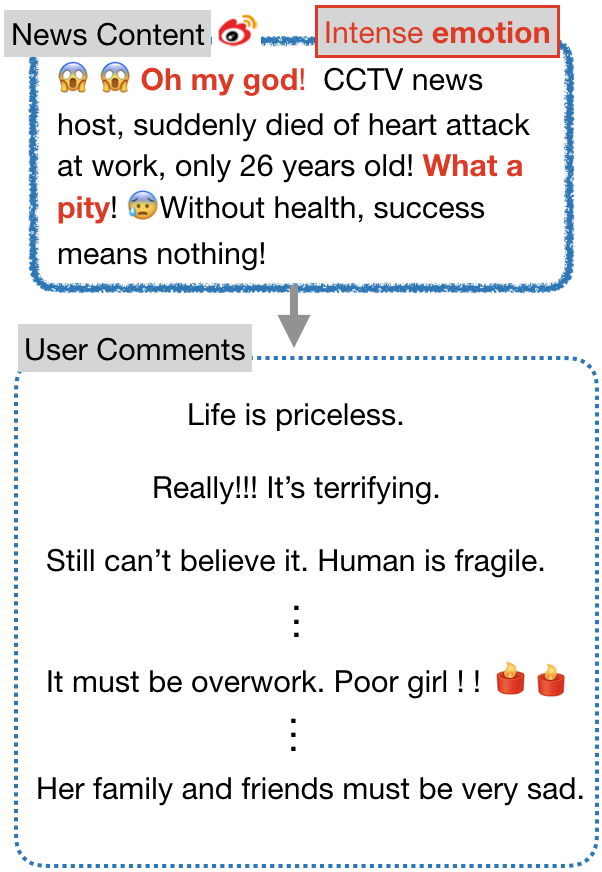
\includegraphics[width=1.66in]{./Figure/introcase1.png}}
		\end{minipage}
		\begin{minipage}[t]{0.225\textwidth}
			\subfloat[]{\label{Fig:introcase2}%%
				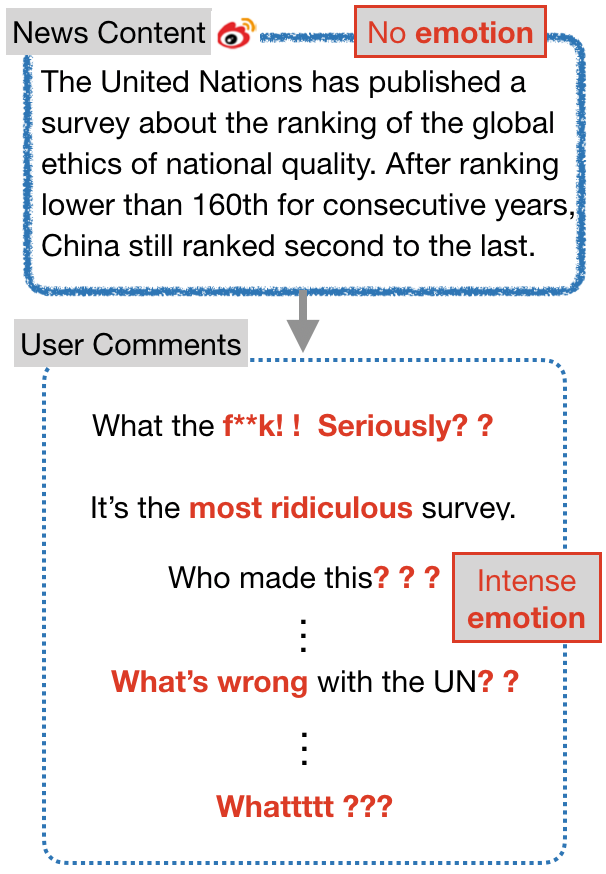
\includegraphics[width=1.67in]{./Figure/introcase2.png}}
		\end{minipage}
		\caption{Two fake news posts from Sina Weibo: (a) a post containing emotions of astonishment and sadness in \textbf{news contents} that easily arouse the audience, and (b) a post which contains no emotion, but  emotions like doubt and anger in \textbf{user comments} by controversial topics.}
		\label{Fig:introcase}
	\end{figure}
	
	%\kai{In the next four paragraphs, the logic should be adjusted. The logic should be like: p2: describing existing work on fake news detection in a objective way, listing 2-3 representative work that you plan to compare in the experiments; p3: summarizing the limitations of existing work or propose your motivation clearly, such as the two scenarios you mentioned in Fig. 1., for each case, highlighting why it is helpful to detect fake newss. P4: summarizing the challenges and framework, and summarize the contributions}
	
	Existing work on fake news detection mainly focuses on {\em news content} and {\em social context}. Feature-based classification models extract basic semantic and emotion features from content, and statistical features from users \cite{castillo2011information}. Propagation-based models construct the relationship network inside the event, and incorporate social conflicting viewpoints towards event in the network \cite{jin2014news,jin2016news}. Recently, deep learning models are proposed to evaluate the credibility of information on social media, which deeply exploits the semantics information from news content\cite{ma2016detecting}. Basic social context features are fused into deep learning models in some studies\cite{guo2018rumor}. However, emotion information, which is crucial for fake news detection, is underutilized in these studies. Few studies leverage emotion in news contents and social context simultaneously for fake news detection.
	
	%However, existing works on fake news detection lack systematical and comprehensive exploration on emotion. Their attempts at utilizing emotion could be categorized to two clusters: 1) mining users' stances towards an event to evaluate the credibility of this event; and 2) extracting statistical emotional features and then incorporate these features in the whole feature sets or the model. Nevertheless, on the one hand, stance mining approaches mainly focus on the viewpoints of users, ignoring the reaction of the publisher which is a crucial indication of the event's credibility as well. And also, stance mining approaches are unable to capture emotions like {\em anxiety, anger, awe, etc}. On the other hand, extracting statistical emotional features highly rely on sentiment dictionaries, which is unreliable and inaccurate when applied on social media, because of the difference of word usage on social media and in real word. Problems such as emotion migration and minor coverage will happen while matching the words on social media with words in sentiment dictionary. Meanwhile, in these emotion feature works, weighted sum of sentiment words is too simple to measure sentiment metrics of a document.
	
	Fake news publishers often aim to spread information extensively and draw wide public attention. Longstanding social science studies demonstrate that the news which evokes high-arousal, or activating (awe, anger or anxiety) emotions is more viral not only in real world but also on social media\cite{stieglitz2013emotions,ferrara2015quantifying,rosnow1991inside,frijda2010impulsive,lazarus1984stress}.  To achieve this goal, fake news publishers commonly adopt two approaches. First, publishers post news with intense emotions which can trigger a high level of physiological arousal in the crowd. For example, in Figure \ref{Fig:introcase1}, the publisher uses rich emotional expressions (e.g., ``Oh my god!'') to make this information more impressive and striking. Second, publishers may present the news objectively to make it convincing but with controversial content which evokes intense emotion in the public, encouraging it spreading widely. As another example (see Figure \ref{Fig:introcase2}) shows, the publisher writes the post in an unemotional way; while, the statement that China ranks second to the last suddenly brings on tension in the crowd, and people express their feeling of anger (e.g., ``most ridiculous''), shock and doubt (e.g., ``seriously?'') in comments.
	% 	and 2) present the news objectively to make it convincing whose content, however, is controversial which evoke intense emotion in the public, and finally spreads widely. Figure \ref{Fig:introcase1} demonstrates the first approach. The publisher uses rich emotional expressions to make this information more impressive and striking. While in Figure \ref{Fig:introcase2}, the publisher writes the post in a unemotional way. However, the statement that China ranks second to the last suddenly bring on tension in the crowd. People express their feeling of anger, shock and doubt in comments. 
	Therefore, learning emotion of the publisher and  users corporately has the potential to improve fake news detection performance.
	% , which is limited in majority of existing studies.
	 
	\new{There exists a realistic dilemma of exploiting emotion. Since a large part of fake news doesn't contain emotional signals in contents, difference of emotion between fake news and real news content may not be obvious. However, fake news content tends to be more controversial and instigating, though unemotional. Hence it is necessary to mine the emotion information from the audience, such as reposts or comments. The majority of existing work utilizing emotion information for detecting fake news either extract emotion feature from news content\cite{castillo2011information,guo2018rumor}, or model the viewpoints of users in propagation\cite{jin2016news, tacchini2017some}.}
	
	To exploit emotion information for fake news detection, we define two types of emotion: (1) \textbf{{\em publisher emotion}}: emotion of the publisher while posting information on social media; and (2) \textbf{{\em social emotion}}: emotion of users when the information disseminates on social media. 
	In this paper, news content and user comments are used to capture {\em publisher emotion} and {\em social emotion}, respectively.  
	In essence, we investigate: (i) how to capture signals of {\em publisher emotion} and {\em social emotion} from news content and user comments, respectively; and (ii) how to exploit publisher and social emotions simultaneously for fake news detection. Our solution to these two challenges is a novel \underline{E}motion-based \underline{F}ake \underline{N}ews Detection framework ({\m}). \new{Technically, we leverage emotion embedding for better emotional representation of each word. And three gate units are designed to exploit information from different modules simultaneously.} Our main contributions are summarized as follows:
	%Firstly, we prove the difference of publisher emotion and social emotion between fake news and real news from various perspectives. A novel end-to-end \underline{E}motion-based \underline{F}ake \underline{N}ews Detection framework(EFN) is proposed which jointly learn the {\em publisher emotion} and {\em social emotion} by two modules: {\em content module} and {\em comment module}, and incorporate emotion with semantic information to detect fake news. 
	
	%Due to the limitations of sentiment dictionary based emotion representation, we leverage a emotion corpus on social media to obtain the emotion representation for each word, which is refereed as {\em emotion embedding} in this paper. To better fuse information from different source for each word or module, we design three {\em gates} which could selectively discard or maintain information from either source. 
	
	%The main contribution of this paper can be summarized as follows:
	\begin{itemize}
		
		\item We provide a principled way to capture the {\em publisher emotion} and {\em social emotion} signals, and demonstrate the importance of these two emotions from various perspectives on fake news detection;
		% 		\item We categorize the emotions on social media as {\em publisher emotion} and {\em social emotion}, and verify the importance of these two emotions on fake news detection.
		\item We propose a novel framework {\m}, which exploits a deep neural network to learn representations from {\em publisher emotion}, {\em social emotion} and content simultaneously, for fake news detection;
		% 		\item We propose a novel framework({\m}) to model the publisher emotion, social emotion and content simultaneously, which can learn emotion
		% 		where {\em emotion embedding} is adopted for better emotion representation and gate mechanism is applied for fusion.
		\item We conduct experiments on real world datasets to show the effectiveness of {\m} for fake news detection. 
		%The result shows that our framework outperforms the existing feature-based methods and state-of-art neural network models.
	\end{itemize}
	
	\new{The paper is organized as follows. In the next section, we give an overview of related. Next, we demonstrate the difference of emotion between fake news and real news with analysis on a dataset. Section IV presents the details of the framework {\m}, including emotion embedding and various gates. Datasets, experiment settings and results are presented in Section V. We conclude our work in Section VI.}
	
	\section{Related Work}
	
	We briefly describe the related work from three-folds: i) Fake News Detection, ii) Emotion Representation, and iii) Multi-modal Fusion.
	
	\subsection{Fake News Detection}
	
	Previous fake news detection studies mostly focus on extracting features and training a classifier to predict the credibility of news. Early work manually extracts a wide range of features including user features, content features, propagation features and topic features\cite{castillo2011information}.  Location and client are proved to be effective in detecting fake news as well\cite{yang2012automatic}; Besides feature-based models, propagation-based approaches aim to mine the relations between various entities in an event. Propagation network is firstly introduced on evaluation in work \cite{gupta2012evaluating}. Tweets, users, events and their inter-relations construct a hierarchical network, which then evaluates the credibility of each tweet and event by iterative calculation. Then, similar structure is applied on microblogs which consists of news, sub-events and messages \cite{jin2014news}. And conflicting viewpoints among users are further investigated in the propagation network\cite{jin2016news}.  Recently, neural network models are adopted for fake news detection. Ma et al.\cite{ma2016detecting} firstly applies RNN for detection on social media by modeling the posts in an event as a sequential time series. Guo et al.\cite{guo2018rumor} proposes a social attention network to capture the hierarchical characteristic of events on microblogs. 
	
	So far,  emotion in these works is used by tools of either emotion features or viewpoints of users, which requires systematical and comprehensive explorations in future work.
	
	\subsection{Emotion Representation}
	
	Early studies primarily use sentiment dictionaries for representing emotion of words. There are several widely-used sentiment dictionaries, including WordNet \cite{wordnet}, LIWC\footnote{www.liwc.net}, MPQA \cite{MPQA}for English, and HowNet~\footnote{http://www.keenage.com/html/e\_index.html} for Chinese. \new{Beyond this, many works leverage these dictionaries and man-made rules to exploit emotion information. For example, Vader\cite{hutto2014vader} constructs a list of lexical features and rules to assess the sentiment of microblog-like contents. However, this method could only align each sentiment word with an emotional class, or intensity value which is somewhat not informative for representing words' emotion. Besides, low coverage and differences of word usage on social media and in real world also limit the effectiveness of sentiment dictionaries in many circumstances. }
	%However, this method may encounter problems of emotion migration and low coverage on social media, because of the differences of word usage on social media and in real word. 
	
	\new{Learning task-specific emotion embedding with neural network could encodes sentiment information in the continuous representation of words, which has been proved to be effective recently. Tang et al.\cite{Tang14} utilizes a massive distant-supervised tweet dataset to obtain emotion embedding on social media.} Agrawal et al.\cite{agrawal2018learning} learns emotion-enriched word-representation on product reviews with a much smaller corpus. \new{This sort of methods enable each word to obtain a distributed representation vector that contains rich and high-level emotion information. }
	
	\subsection{Multimodal Fusion}
	The simplest approach is concatenation. Silberer et al.\cite{silberer2017visually} employs a stacked autoencoder to learn multimodal representations by embedding linguistic and visual inputs into a common space. However, these methods treat the different modalities equally in fusion. In work \cite{jin2017multimodal}, the authors employ the high-level representation of visual modal as an external attention vector to weigh the components of textual modality. Gate mechanism is also widely used in many fusion works. LSTM \cite{hochreiter1997long} and GRU \cite{bahdanau2014neural} tackle the long-term dependency problems of RNN with different gates that could control how information from last time step and current inputs updates at current unit, which is another form of fusion. Wang et al.\cite{wang2018learning} uses gate units to learn the weights of different modal representations for each word. 
	
	Considering the importance of emotion in fake news detection, we propose a novel fake news detection framework which could exploit emotion information from publisher and users with the help of emotion embedding and gate units.
	
	
	\section{A Preliminary Analysis on Emotion Signals }\label{sec:analysis}
	To explore the relationships between emotions and fake news on social media, we perform a preliminary data analysis on emotions signals for fake and real news in news content and user comments respectively. We collect the dataset from a popular microblog platform Weibo~\footnote{www.weibo.com} (details of data preparation are introduced in Sec~\ref{sec:data}). We have collected 7,880 fake news pieces and 7,907 real news pieces, and their related user comments. The analysis is performed from three perspectives: 1) the emotional category; 2) the emotional intensity; and 3) the emotional expression.
	
	\subsection{Emotional Category}
	%\kai{Use 1-2 sentences to explain WHY emotion categories are compared here}
	Generally, fake news is sensational and inflammatory. It could arouse specific kinds of emotions among the users such as suspicion, anxiety or shock. Therefore, we select 5 fine-grained emotional categories to investigate emotions in fake and real news, including \textit{anger}, \textit{sadness}, \textit{doubt}, \textit{happiness} and \textit{none} (Some contents may not contain emotional information). We adopt the classifier in Sec~\ref{sec:classifier} to annotate our experimental data with emotion categories. 
	
	Figure \ref{Fig:ec1} and \ref{Fig:ec2} exhibit the distribution of emotional categories in news content and user comments respectively. In fake news' content, the proportion of \textit{anger} is 9\% higher than it in real news’, while the percentage of \textit{happiness} is 8\% lower. Same trend happens in the user comments. In addition, the proportion of sadness in fake news' contents and doubt in fake news' comments is much higher than them in real news.  This result demonstrates that, compared to in real news, both the publisher and users tend to express more high-arousal emotions in fake news.
	
	\begin{figure}[h]
		\centering
		
		%大图:0.44,3.25in
		\begin{minipage}[t]{0.24\textwidth}
			\subfloat[News Content]{\label{Fig:ec1}%%
				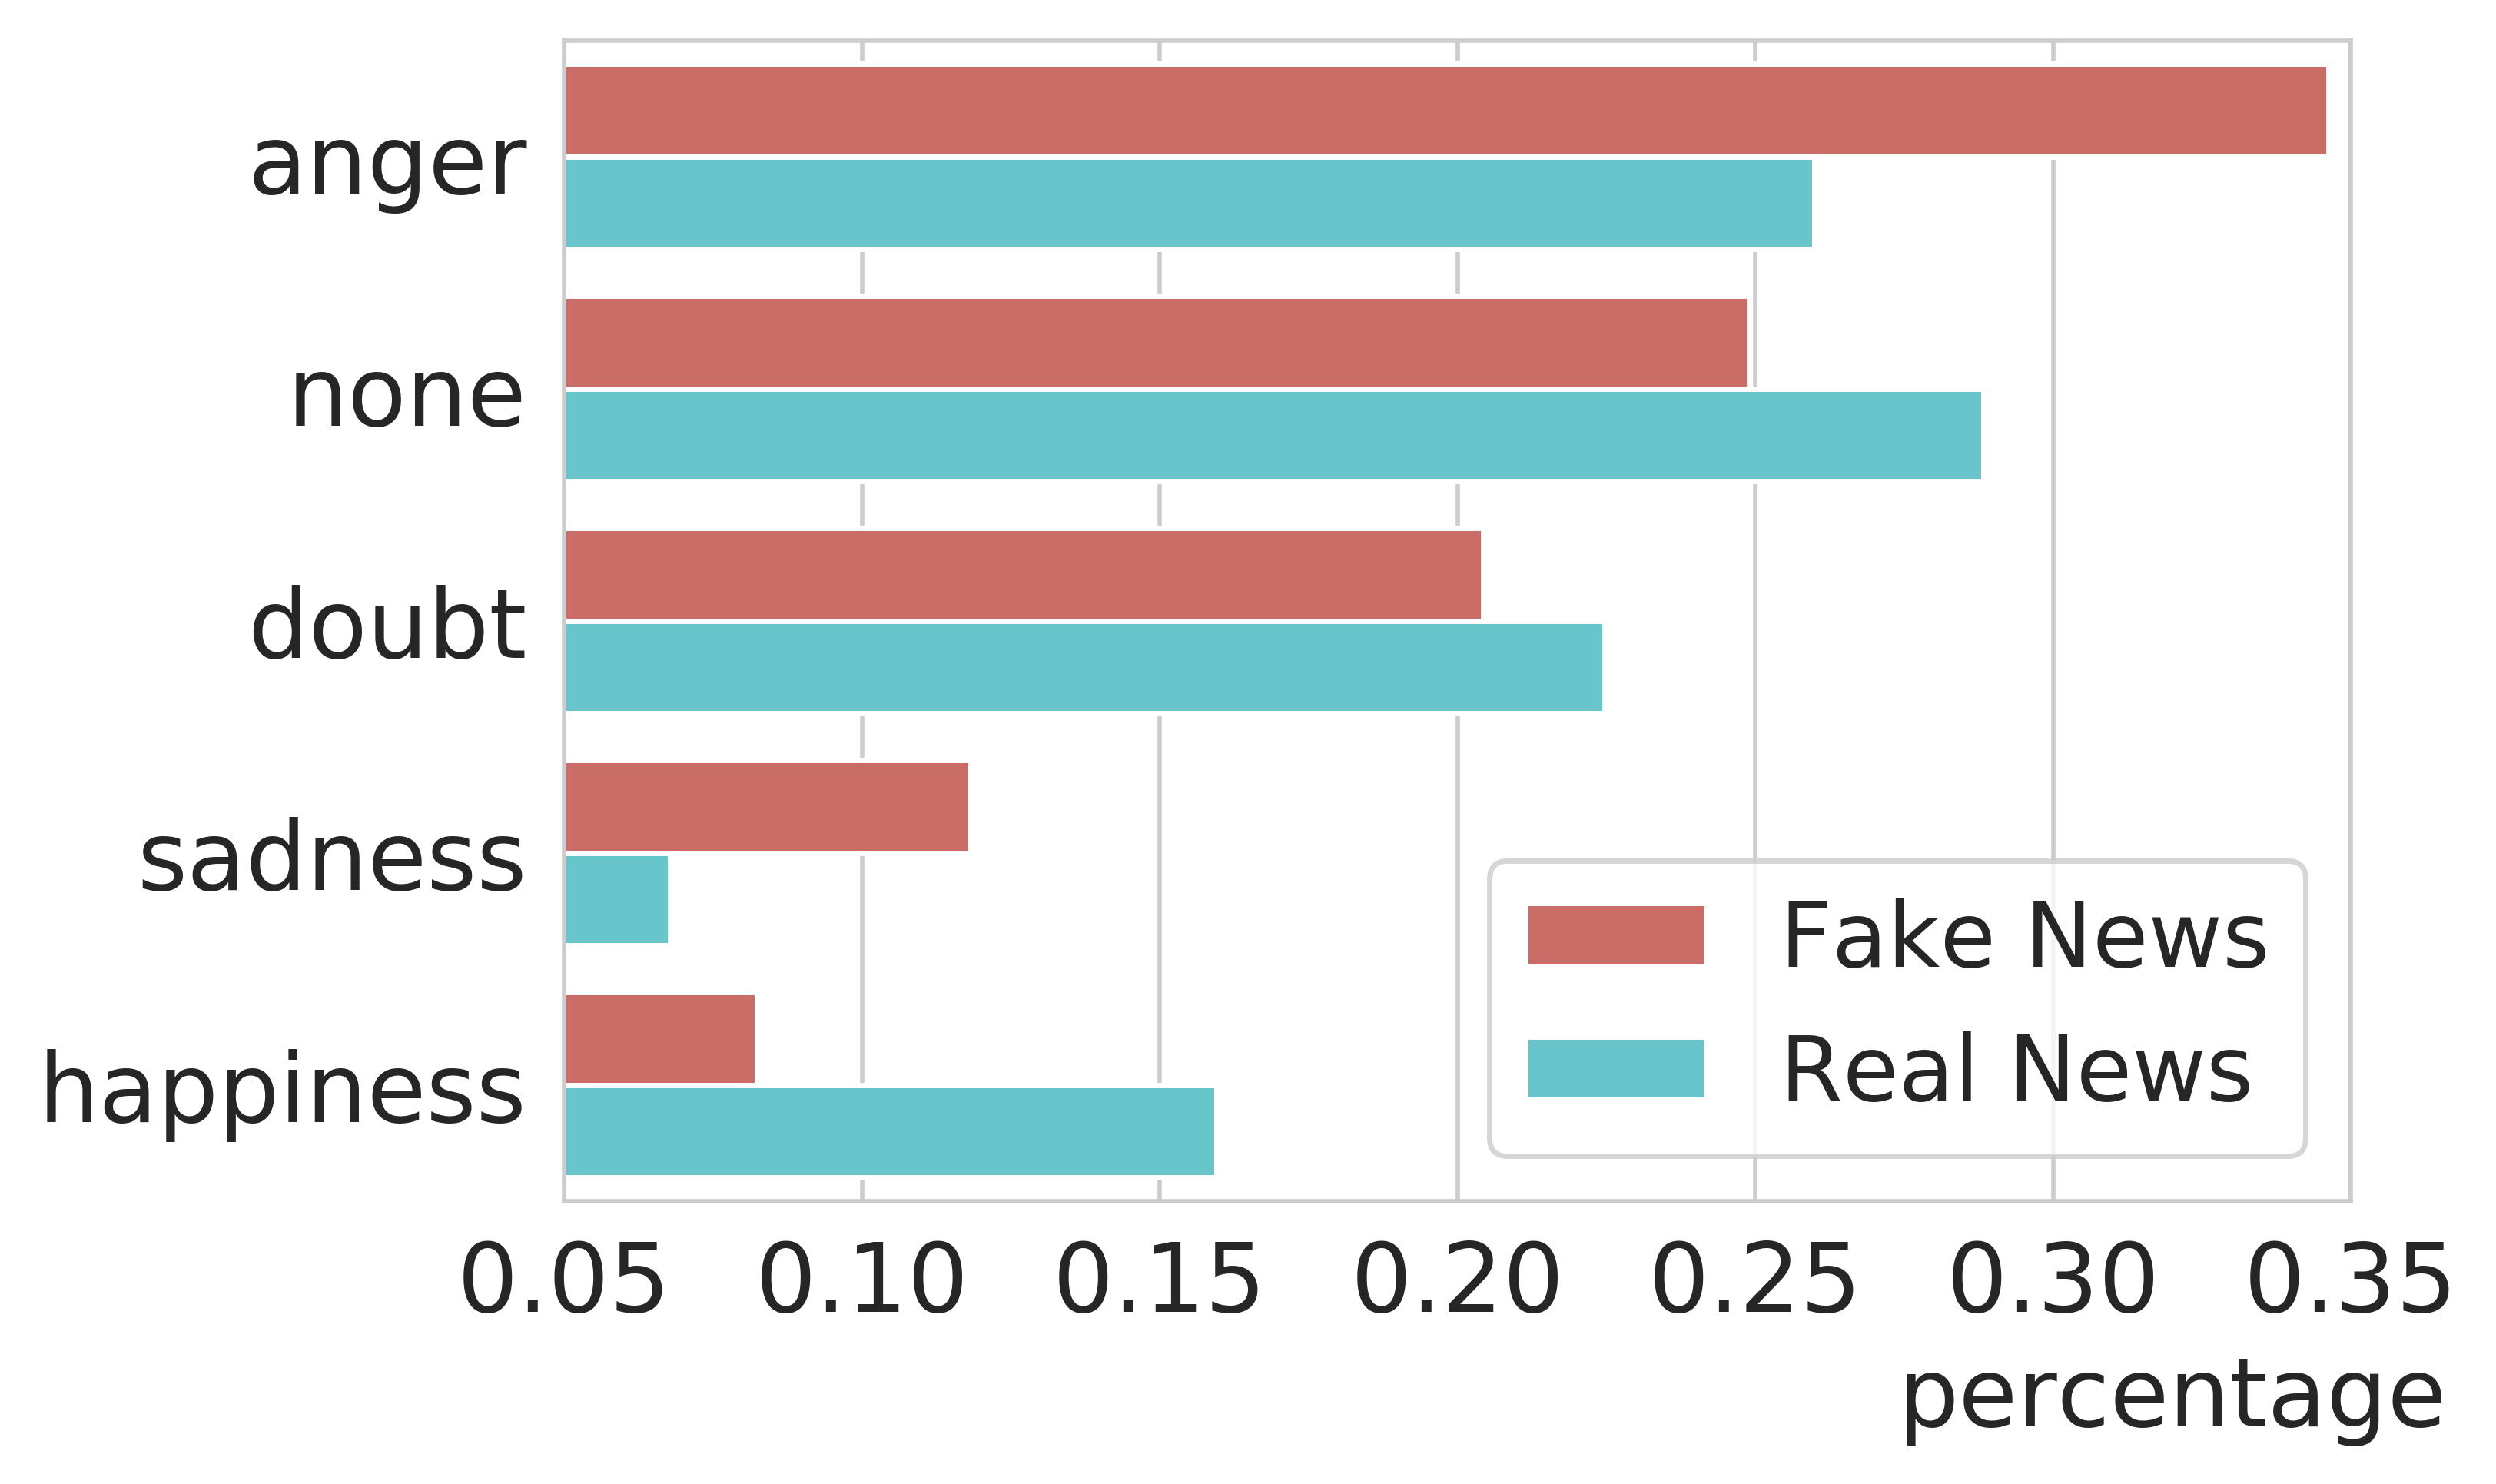
\includegraphics[width=1.75in]{./Figure/emotion-category-main.png}}
		\end{minipage}
		\begin{minipage}[t]{0.24\textwidth}
			\subfloat[User Comments]{\label{Fig:ec2}%%
				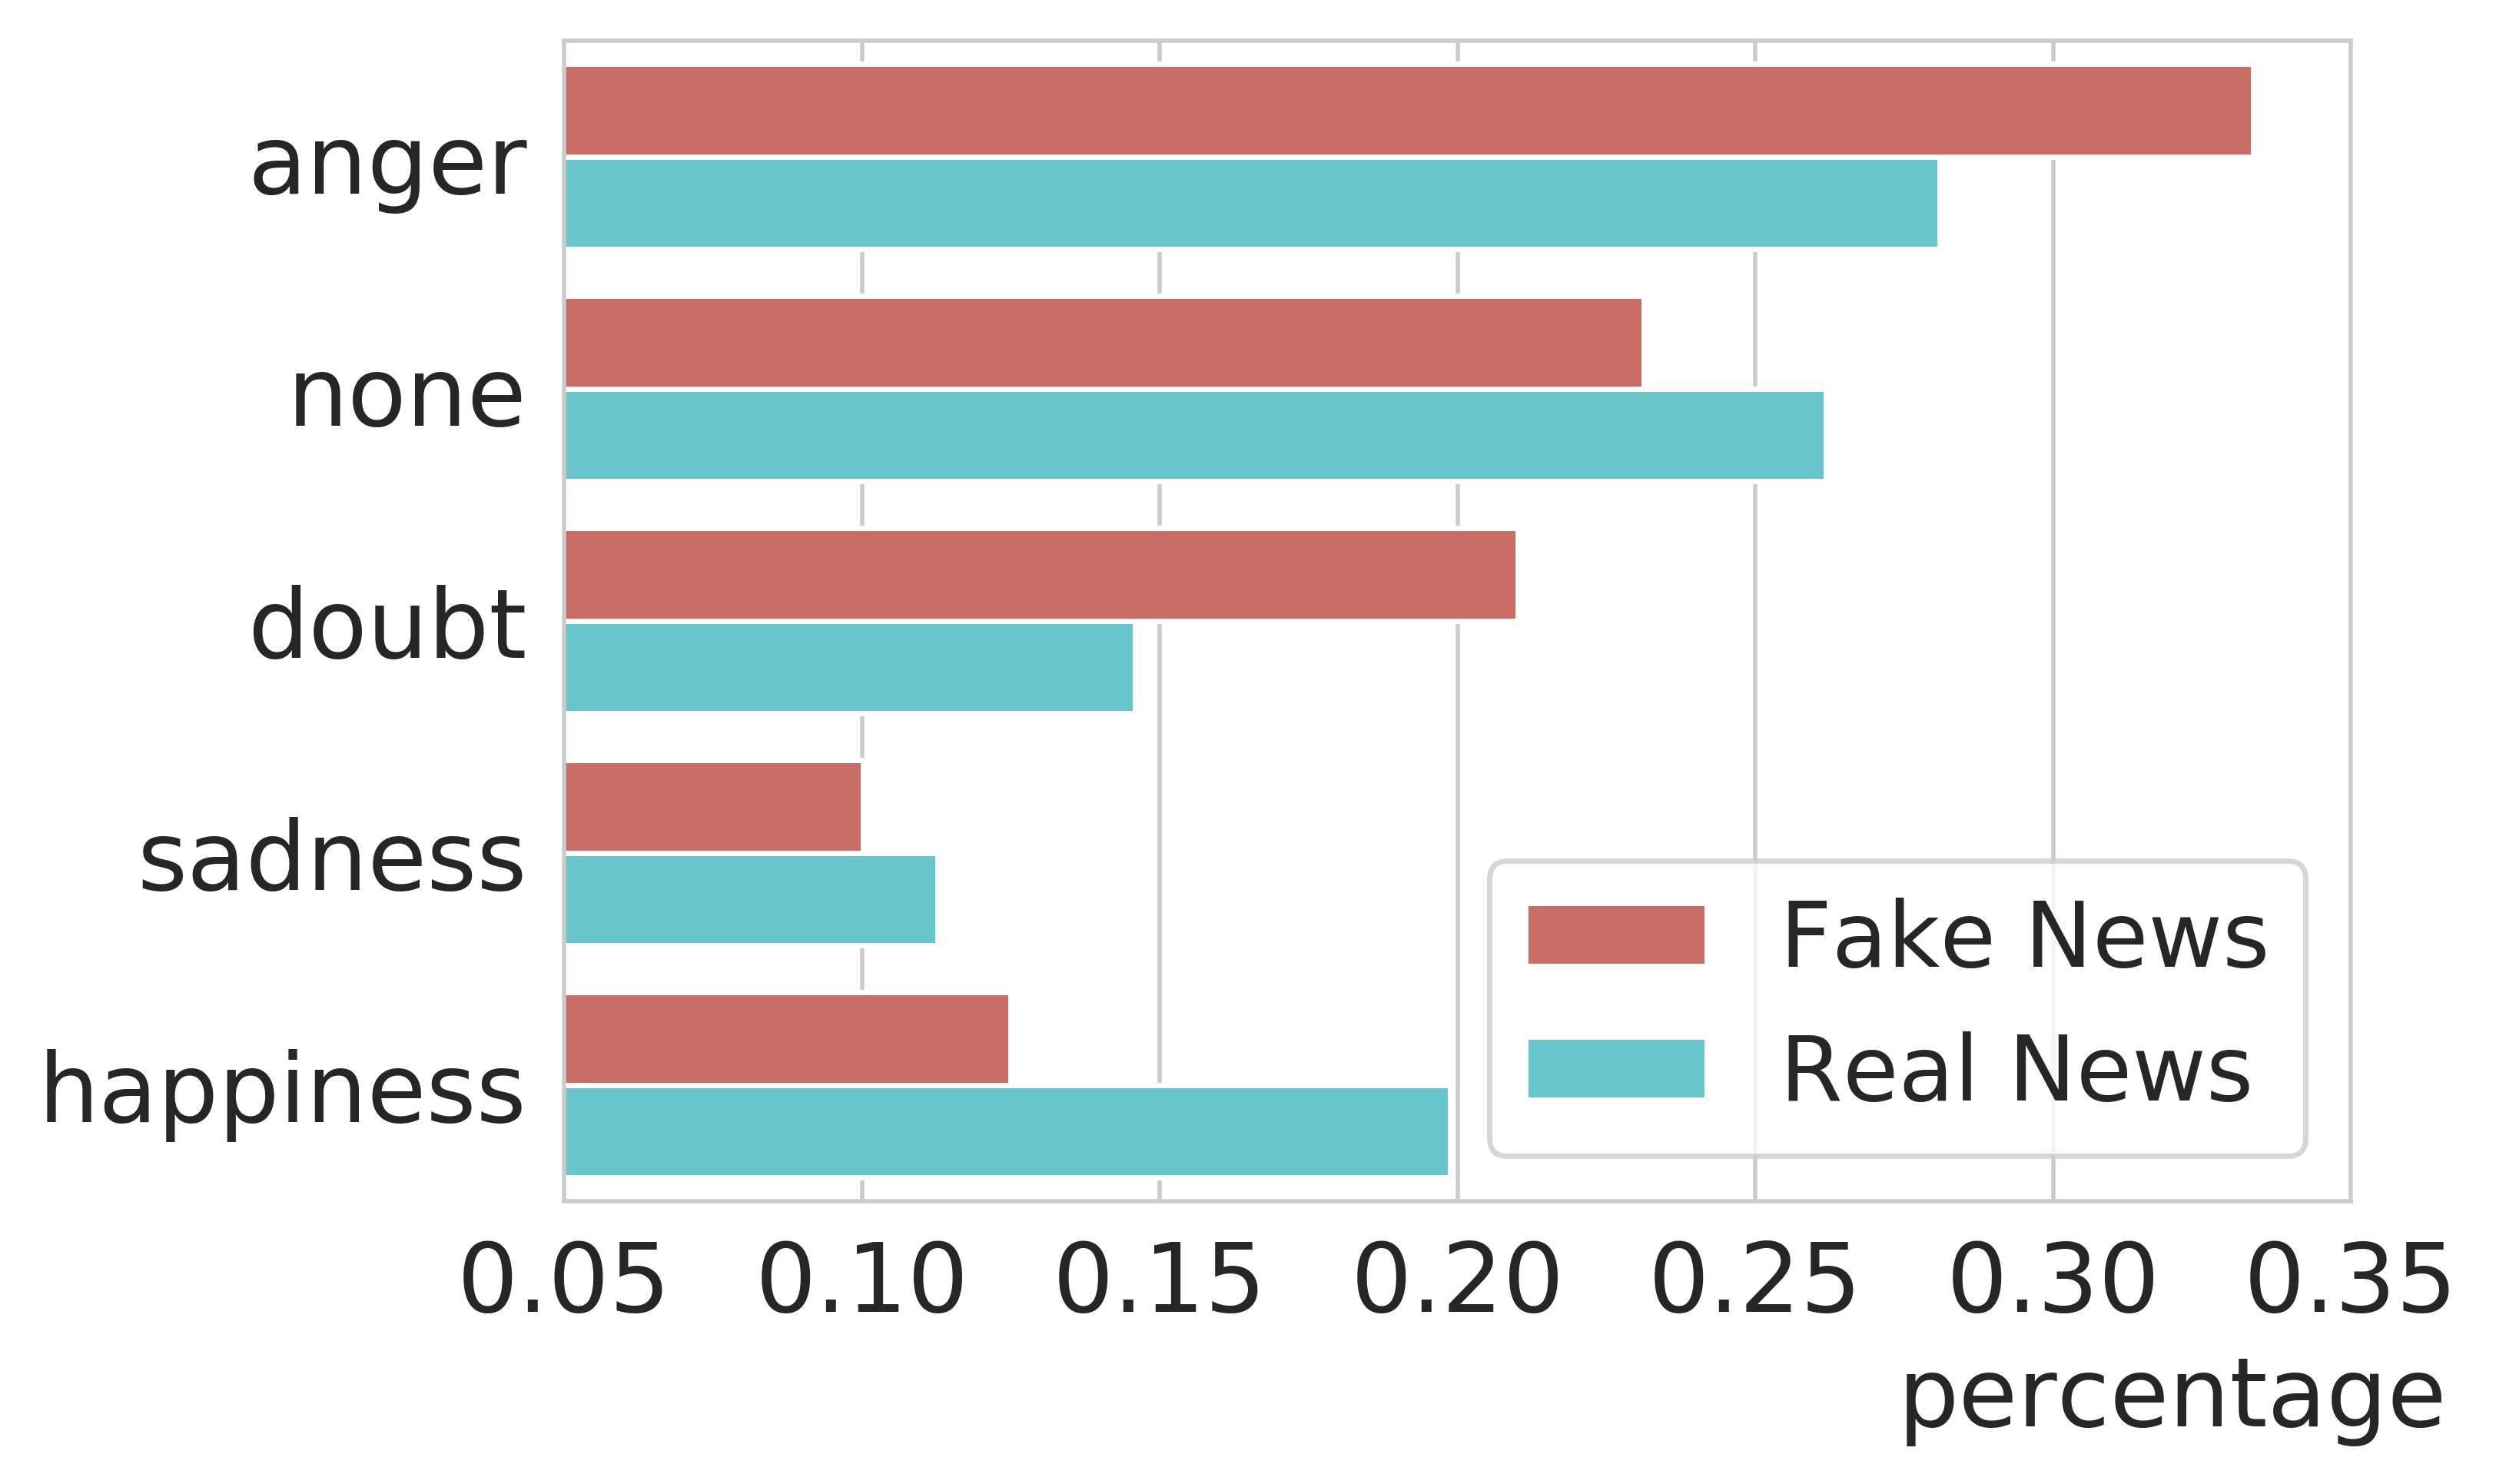
\includegraphics[width=1.75in]{./Figure/emotion-category-comments.png}}
		\end{minipage}
		
		\caption{Distributions of emotional category of fake news and real news in: (a) news content and (b) user comments. {\em Anger} is more likely to appear in fake news, while real news arouse more {\em happy} emotion in both sources}
		\label{Fig:emotionCategories}
	\end{figure}
	
	\subsection{Emotional Intensity}
	%\kai{Use 1-2 sentences to explain WHY emotion intensity are compared here; add one sentence to explain what is emotion intensity}
	%According to our assumption, the content emotion of rumor events and their emotion evoked in crowds, which we define as social emotion, tend to be quite intense to impress the audience and spread extensively. Hence we explore the emotional intensity of rumor to make it solid.
	
	Each document also owns an emotional intensity level in each emotional category. For example, the intensity of {\em I'm super happy} is much stronger than intensity of {\em I'm happy} in emotional category {\em happiness}. Fake news is expected to express negative emotion with stronger intensity which could further arouse intense emotions in the public. In this section, we take the output probability of emotional category classifier\\’s(in Sec~\ref{sec:classifier}) softmax layer as the emotional intensity level for each emotional category, which is a continuous value between 0 and 1.
	
	In Figure \ref{Fig:emotionalIntensity}, we can see that, regardless of sources, the emotions of \textit{anger}, \textit{sadness} and \textit{doubt} in fake news are much  severer than in real news. And this discrepancy is more drastic in news content. In conclusion, both the publisher and users are more possible to express stronger negative emotions in fake news than in real news, while the trend of positive emotion is reverse.
	\begin{figure}[h]
		\centering
		
		% 大图:0.44,2.75in
		\begin{minipage}[t]{0.24\textwidth}
			\subfloat[News Content]{\label{Fig:ei1}%%
				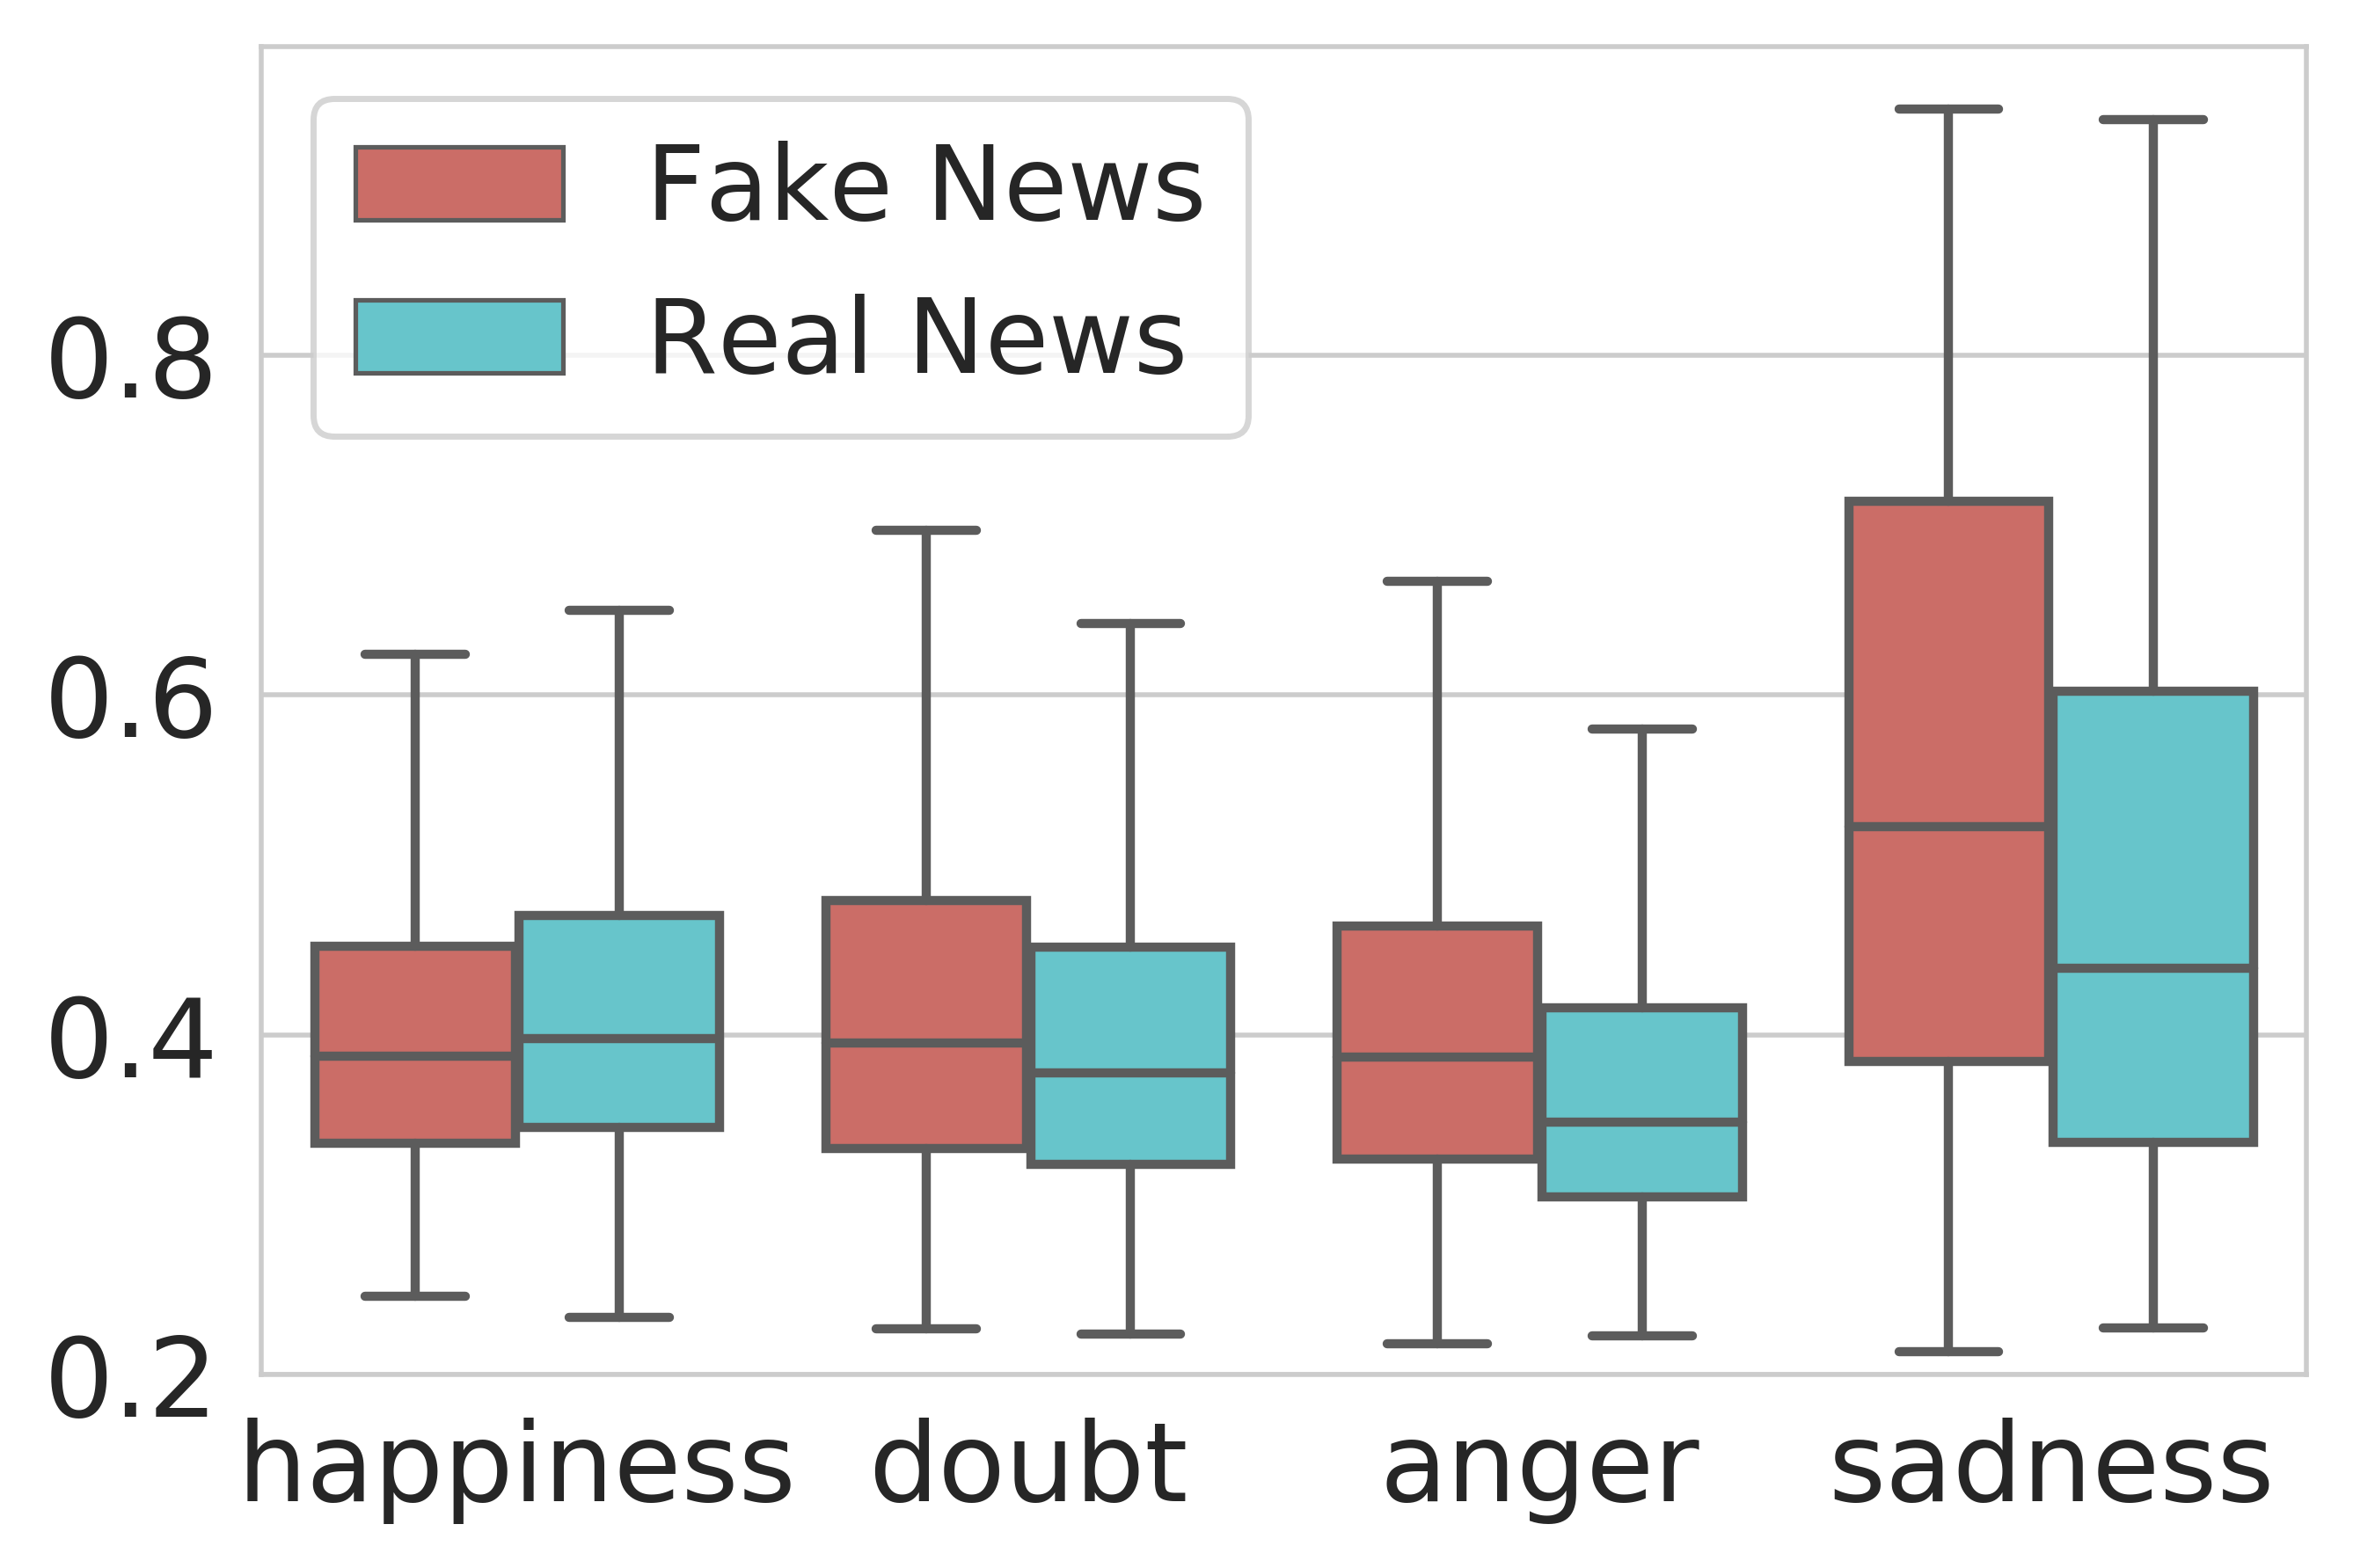
\includegraphics[width=1.75in]{./Figure/emotion-intensity-main.png}}
		\end{minipage}
		\begin{minipage}[t]{0.24\textwidth}
			\subfloat[User Comments]{\label{Fig:ei2}%%
				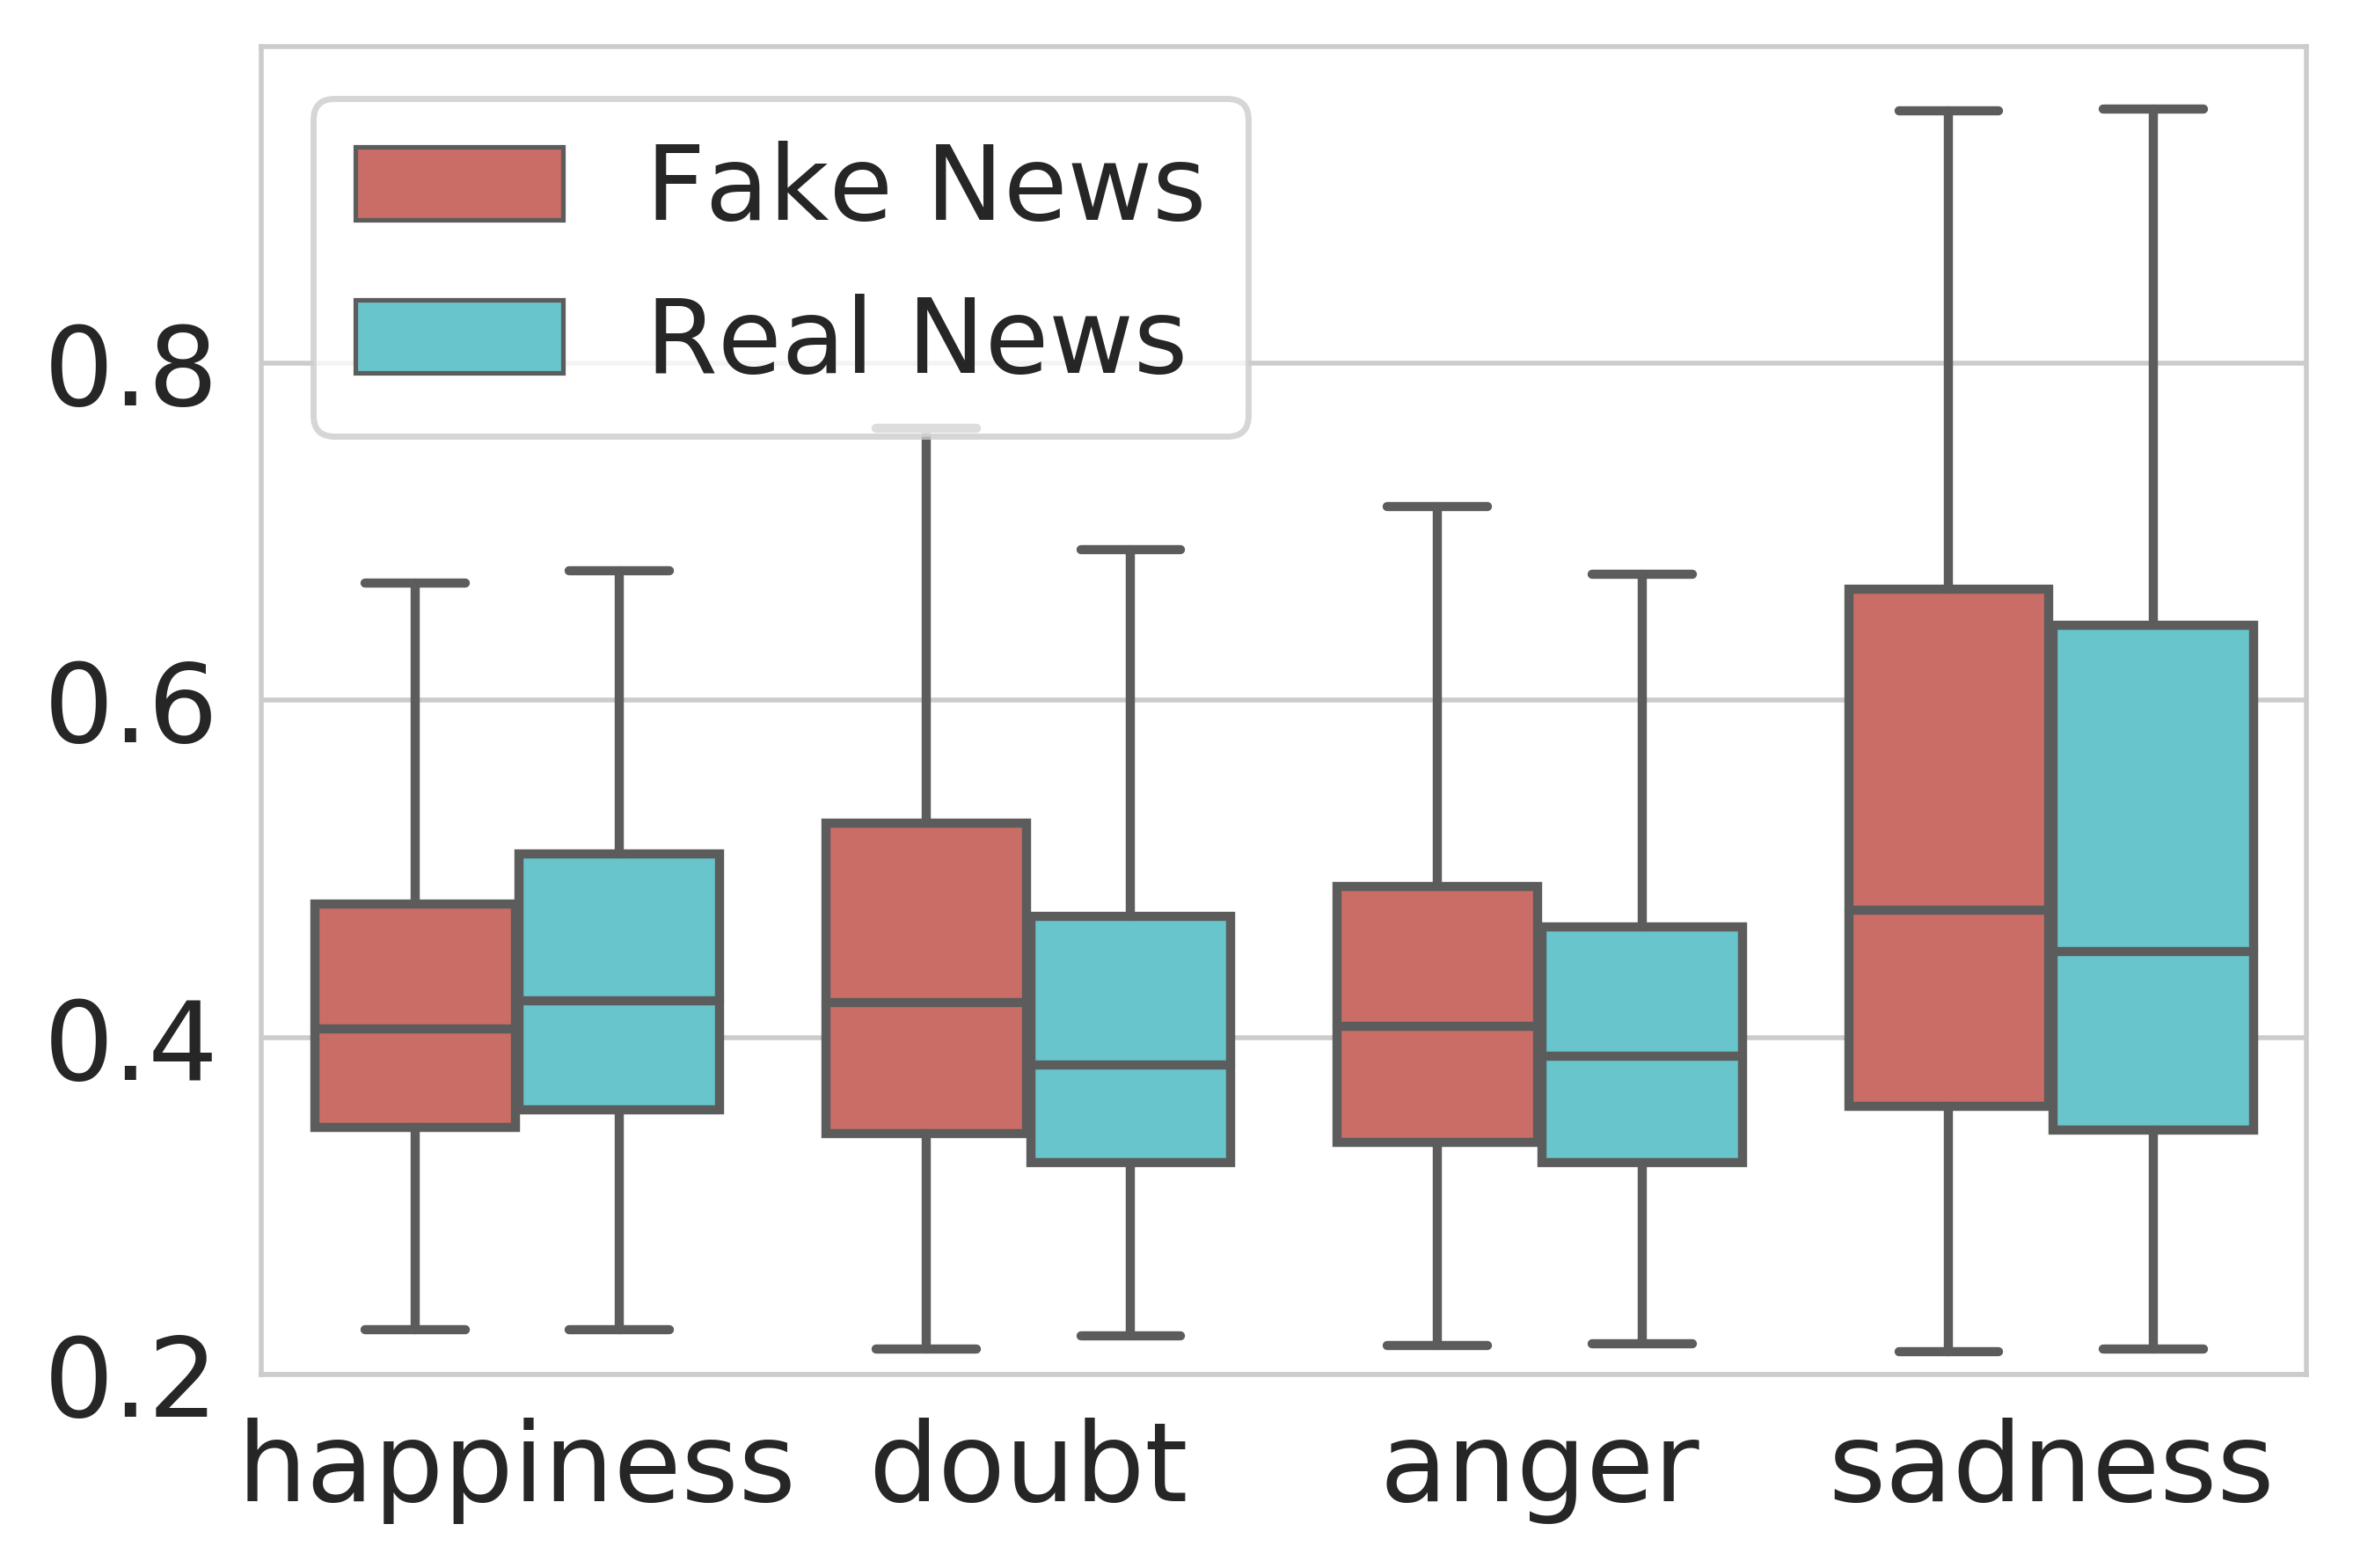
\includegraphics[width=1.75in]{./Figure/emotion-intensity-comments.png}}
		\end{minipage}
		
		\caption{Distributions of emotional intensities level of fake news and real news in: (a) news content and (b) user comments. The intensities of emotion \textit{anger}, \textit{sadness} and \textit{doubt} in fake news are all stronger than in real news.}
		\label{Fig:emotionalIntensity}
	\end{figure}
	
	\subsection{Emotional Expression}
	%\kai{Use 1-2 sentences to explain WHY emotion expression are compared here}
	%The analysis above has revealed that the distributions of emotion categories of fake news and Non-Rumor gap a lot. Moreover, we extract the differences of emotional vocabulary expression between the two for same kinds of emotion.
	
	Different people may express their feelings with different linguistic usage. For example, some people like using plain words to express their feelings, while others prefer exaggerated words. In fake news, inciting words might be more preferred. To analyze the differences of emotional expression, we extract the top-weighted words for expressing {\em anger} in real news and fake news respectively. We adopt the widely-used method in \cite{nlpcc14} to calculate the weight of each word in the dataset. 
	%The weights is positively correlated with the word's frequency in this emotion category, and negatively correlated with its frequency in other emotion categories and in the whole dataset. 
	%In practice, we mix the top words in news content with their comment, because the their top words are similar. 
	The top-weighted 30 words in fake news and real news are shown in Figure \ref{Fig:emotionalExpression}. 
	\begin{figure}[h]
		\centering
		
		\begin{minipage}[t]{0.24\textwidth}
			\subfloat[Fake News]{\label{Fig:ee1}%%
				\includegraphics[width=1.75in]{./Figure/words-rumor-anger.png}}
		\end{minipage}
		\begin{minipage}[t]{0.24\textwidth}
			\subfloat[Real News]{\label{Fig:ee2}%%
				\includegraphics[width=1.75in]{./Figure/words-truth-anger.png}}
		\end{minipage}
		
		\caption{Emotional expressions for \textit{anger} in fake news and real news. Compared to real news, fake news use more fierce and extreme words to express {\em anger}.}
		\label{Fig:emotionalExpression}
	\end{figure}
	
	We can see that fake news conveys \textit{angry} with much more fierce and extreme words like {\em "damn it", "ass"}. Similar circumstance also exists in other negative emotional categories. Therefore, people use different words for emotional expression in fake and real news.
	
	In summary, we make the following conclusions from these experiments: i) both the publishers and users are more likely to spread more negative emotions in fake news than in real news; ii) participants of fake news tend to express negative emotions with stronger intensities; and iii) while expressing a specific kind of emotion, people in fake news prefer exaggerated and inflammatory words. 
	%Therefore, exploiting emotion would be great helpful for detecting fake news on social media.
	
	\section{Modeling Emotions for Fake News Detection}
	
	In this section, we present the details of  the proposed end-to-end emotion based fake news detection framework {\m}. It consists of three major components (see Figure~\ref{Fig:framework}): i) the content module exploits the information from the publisher, including semantic and emotion information in news contents;  ii) the comment module captures semantic and emotion information from users; and iii) the fake news prediction component fuses the high-level features from news content and user comments, and then classify it as fake or not. 
	% 	The whole framework is trained end-to-end.
	
	\subsection{Content  Module}
	News contents contain the cues to differentiate fake and real news. We have shown that the distributions of emotional categories are different for fake and real news pieces, which demonstrate the potential to use news content emotions to help detect fake news. 
	
	% Content module in this paper aim to learn the information from the publisher, especially the semantic information and emotion information of the source posts. Figure \ref{Fig:contentmodule} demonstrate the structures of content module. We employ bidirectional gated recurrent unit network(BiGRU)\cite{bahdanau2014neural} to learn the high-level representation of semantic and emotion, and even the content module. GRU is a refined recurrent neural network which is proposed by \cite{bahdanau2014neural}, where the reset gate $r_t$ and update gate $z_t$ together control how information is updated to the state. Bidirectional structure enable each state to capture information from both previous and subsequent context information. BiGRU has been widely applied in many natural language processing tasks, such as text classification, machine translation, question answering, etc. And a gate {\em gateT} is used on each word, transferring the three inputs: emotion embedding, word embedding and sentence emotion features to a new low dimensional continuous vector. 
	
	% In detail, each word would be represented as two embedding vector, one is word embedding and another is emotion embedding. The word embedding vector for each word is initialized with the pre-trained word2vec\cite{mikolov2013distributed} on a given datasets. And the emotion embedding is initialized with the embedding vectors which is extracted from the embedding layers that described in section 4.1. Let $ P = \{p_1, ...,p_N\}$ denote the source posts in the datasets. And let $T = \{t_1, ...t_M\}$ be the words of a post, where $t_i$ represent $i$-th word in this post. Their corresponding emotion embedding and word embedding representation are $T_e = \{t_1^e, ...,t_M^e, t_i^e \in \mathbb{R}^k\} $ and $T_w = \{t_1^w, ..., t_M^w, t_i^w \in \mathbb{R}^l\}$, as the dimensions of emotion embedding and word embedding vectors are $k$ and $l$ respectively.
	\begin{figure*}[t]
		\centering
		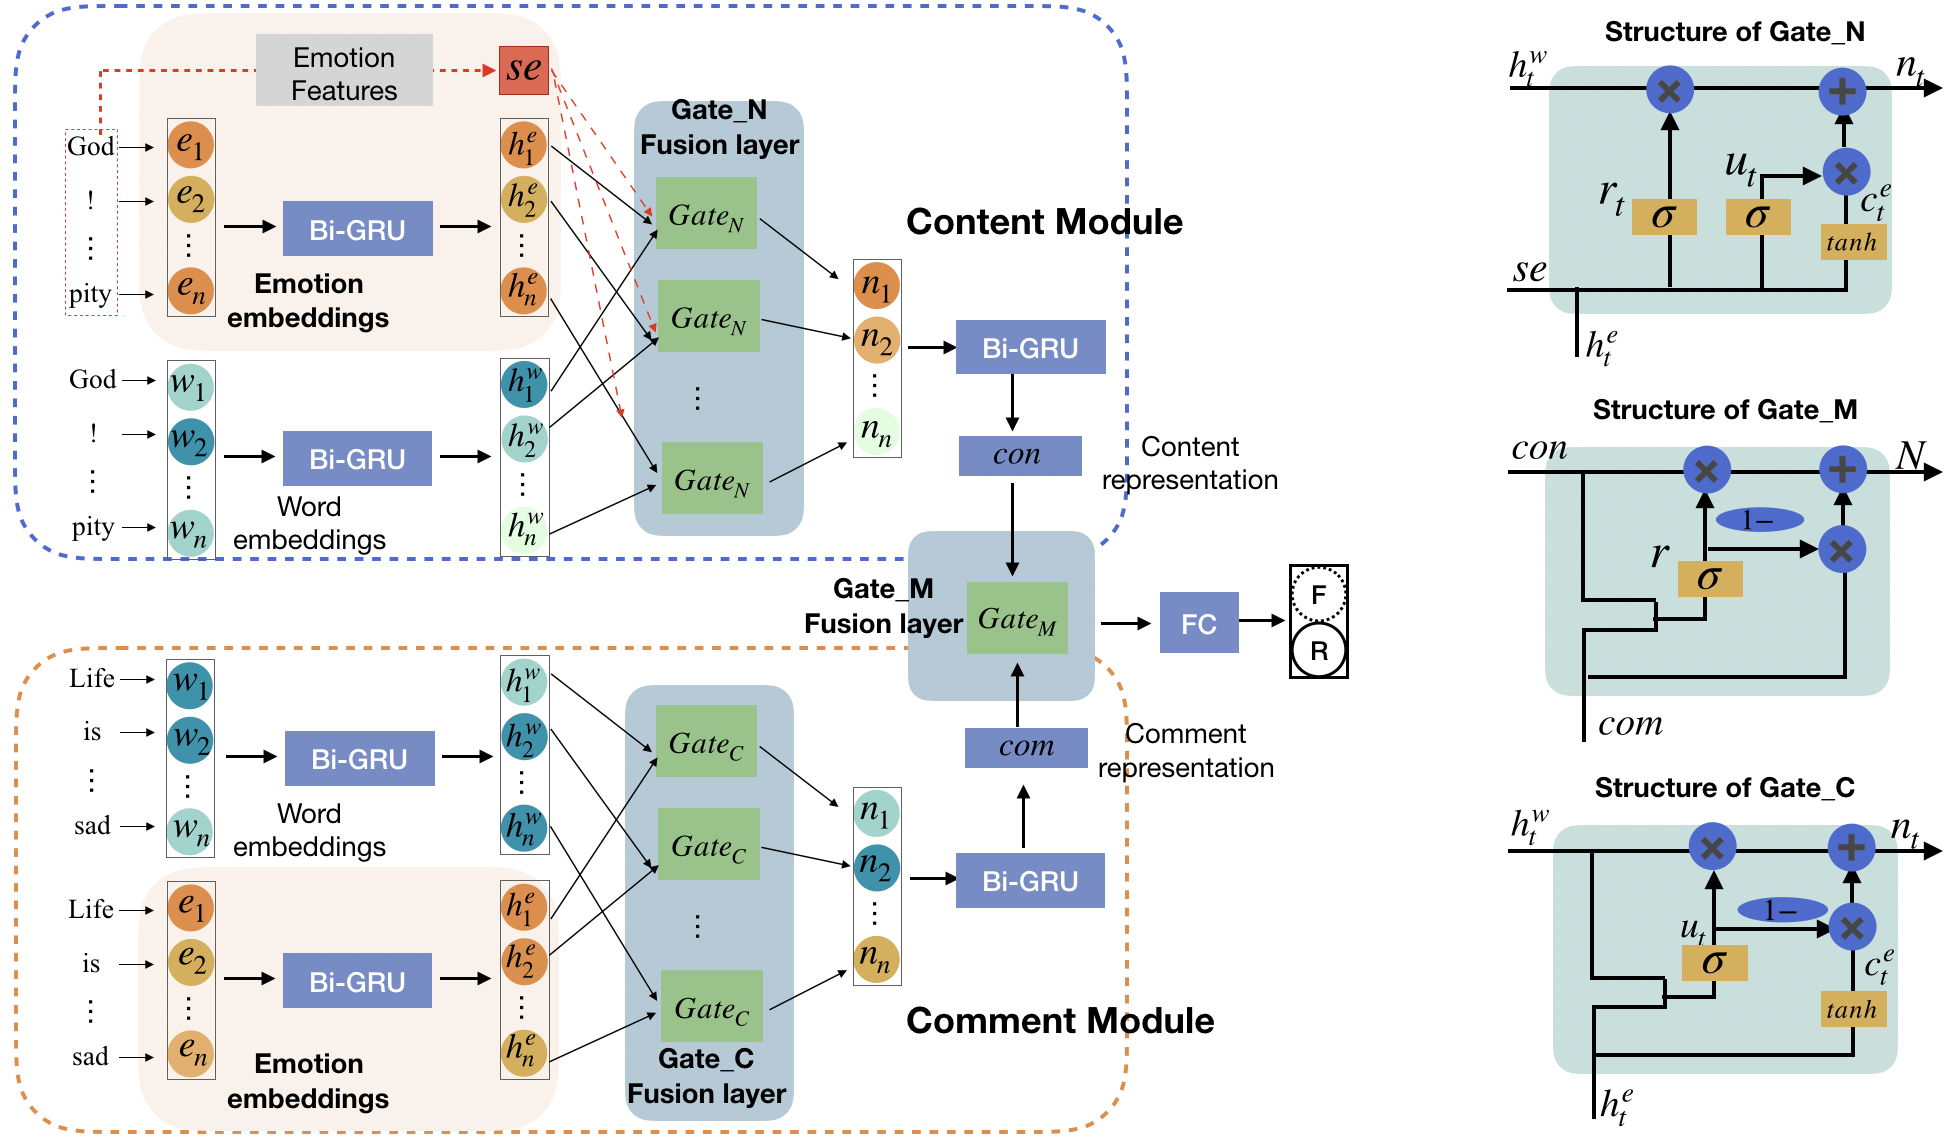
\includegraphics[width=0.8\textwidth]{./Figure/framework.png}
		\caption{The proposed framework {\m} consists of three components: (1) the news content module, (2) the user comments module, and (3) the fake news prediction component. The previous two modules are used to model semantic and emotions from the publisher and users respectively, while prediction part fuses information from these two modules and makes prediction. Three gates at the right side are used for multimodal fusion at different layers in this framework.}
		\label{Fig:framework}
	\end{figure*}
	\paragraph{Word Encoder}
	We learn the basic textual feature representations through a recurrent neural network(RNN) based word encoder. Though in theory, RNN is able to capture long-term dependency, in practice, the old memory will fade away as the sequence becomes longer. To make it easier for RNNs to capture long-term dependencies,
	Gated Recurrent Units (GRU)~\cite{bahdanau2014neural} are designed in a manner to have more persistent memory. To further capture the contextual information of annotations, we use bidirectional GRU to model word sequences
	from both directions of words. For each word $t_i$, the word embedding vector $w_i$ is initialized with the pre-trained word2vec\cite{mikolov2013distributed}. The bidirectional GRU contains the forward GRU $\overrightarrow{f}$ which reads each sentence from word $t_0$ to $t_n$ and a backward GRU $\overleftarrow{f}$ which reads the sentence from word $t_n$ to $t_0$:
	
	% Each sentence in the news source post could be represented as a word embedding matrix by sequentially concatenating the word embedding vectors. We firstly use a bidirectional GRU\cite{bahdanau2014neural} to encode each word to a higher level representation, by summarizing contextual information from both directions for words. The bidirectional GRU contains the forward GRU and backward GRU:
	\begin{equation}
	\begin{aligned}
	\overrightarrow{h_i^w} = \overrightarrow{GRU}(w_i), i \in [1, n],\\
	\overleftarrow{h_i^w} = \overleftarrow{GRU}(w_i), i\in [1, n].
	\end{aligned}
	\end{equation}%
	for a given word $t_i$, we could obtain its word encoding vector $h_i^w$ by concatenating the forward hidden state $\overrightarrow{h_i^w}$ and backward hidden state $\overleftarrow{h_i^w}$, i.e., $h_i^w=[\overrightarrow{h_i^w}, \overleftarrow{h_i^w}]$
	
	\paragraph{Emotion Encoder}\label{sec:classifier}
	Similar to the word encoder, we adopt bidirectional GRU to model the emotion feature representations for words. To preserve the emotion signal for each word, we first introduce how to obtain an emotion embedding vector $e_i$ for each word $t_i$.
	
	Inspired by recent advancements on deep learning for emotion modeling~\cite{agrawal2018learning}, we train a recurrent neural network to learn the emotion embedding vectors. Following traditional settings~\cite{hu2013unsupervised}, we first obtain a large-scale Weibo dataset in which each Weibo contains emoticons. \new{Then we categorize the top 200 emoticons into 5 emotional classes(\textit{anger}, \textit{doubt}, \textit{happiness}, \textit{sadness} and \textit{none} ), and use the emoticons to label the corpus. Next, we initialize each word with the one-hot vector. Here, we don't use pre-trained word embeddings for not learning too much semantic information in emotion embeddings. After initiation, all words pass an embedding layer which projects each word from the original one-hot space into a low dimensional space, and then are sequentially fed into a one-layer GRU model. Finally, through back-propagation, the embedding layer gets updated during training, producing emotion embedding $e^i$  for each word $t_i$. Besides, this classifier is also used for analysis in Sec~\ref{sec:analysis}. For experiment on Twitter, we perform the same procedure on the labeled sentiment tweet corpus which is published in SemEval 2018\cite{SemEval2018Task1} to get emotion embeddings of English words.}
	
	After we obtain the emotion embedding vectors, we can learn the emotion encoding $h_i^e$ for word $t_i$:
	\begin{equation}
	\begin{aligned}
	\overrightarrow{h_i^e} = \overrightarrow{GRU}(e_i), i \in [1, n],\\
	\overleftarrow{h_i^e} = \overleftarrow{GRU}(e_i), i\in [1, n].
	\end{aligned}
	\end{equation}%
	for a given word $t_i$, we could obtain its emotion encoding vector $h_i^e$ by concatenating the forward hidden state $\overrightarrow{h_i^e}$ and backward hidden state $\overleftarrow{h_i^e}$, i.e., $h_i^e=[\overrightarrow{h_i^e}, \overleftarrow{h_i^e}]$.
	
	% Emotion encoder is almost the same as the word encoder. Similarly, we could obtain the emotion encoding vector $h_i^e$ for word $t_i$. Note that the dimension of $h_i^w$ and $h_i^e$ might be different.
	
	\paragraph{Hand-crafted News Emotion Features}
	%\kai{Describe WHY news emotion features are important in few sentences}
	The overall emotion information of news content is also important while deciding how much information from emotion part should be absorbed for each word. For example, the news content which obviously expresses intense emotions could further strengthen the importance of emotion part in each word of the content. For a given post $p_j$, we extract the emotion features included in work \cite{castillo2011information} and also add some extra emoticon features. There are 19 features regarding emotion aspects of news, including {\em numbers of positive/negative words, sentiment score}, etc. News emotion features of $p_j$ is denoted as $se_j$.
	\paragraph{News Content Representation}
	%\kai{Move the content of ``Structure of T\_Gate`` to here and reorganize}
	Gate\_N is applied to learn information jointly from word embedding, emotion embedding and sentence emotion features, and then yield a new representation for each word(see Figure \ref{Fig:framework}). The units in Gate\_N is motivated by the \textit{forget gate} and \textit{input gate} in LSTM. In Gate\_N, two emotion inputs corporately decide the value of $r_t$ and $u_t$ with two sigmoid layers, which are used for managing how much information from semantic and emotion is added into the new representation. Meanwhile, a tanh layer transfer the emotion inputs to the same dimensional space with word embeddings'. Mathematically, the relationships between inputs and output of Gate\_N are defined as the following formulas:
	
	\begin{equation}
	\begin{aligned}
	&r_t = \sigma(W_r.[se, h^e_t] + b_r)\\
	&u_t = \sigma(W_u.[se, h^e_t] + b_u)\\
	&c_t^e = tanh(W_c.[se, h^e_t] + b_c)\\
	&n_t = r_t * h^w_t + u_t * c_t^e\\
	\end{aligned}
	\end{equation}
	
	All the generated vectors of words are fed into a bidirectional GRU layer sequentially, and then the last hidden state of the GRU layer is expected to contain all the information in {\em Content Module}, called {\em Content Representation}.
	
	\subsection{Comment Module}
	%\kai{Move the content of ``Structure of S\_Gate`` to here and reorganize}
	Comment module explores the semantic and emotion information from users in the event. The architecture of comment module is similar to content module's except: 1) all comments are firstly concatenated before fed into BiGRU; 2) there is no sentence emotion features; and 3) Gate\_C is used for fusion.
	
	\new{We choose to concatenate all the comments for inputs because over 70\% news pieces own less than 5 comments, which reflect the situation in real world as well. As a consequence of concatenation, the input doesn't own the intact information as a {\em sentence}, so there is no {\em sentence emotion features}.}
	
	Gate\_C is introduced for fusion in comment module. Different from Gate\_N, there are only two input modalities. We adopt the \textit{update gate} in GRU to control the update of information in fusion process (see Figure \ref{Fig:framework}). Two inputs jointly yield a update gate vector $u_t$ through a sigmoid layer. A tanh layer create a vector of new candidate values, $c_t^e$, which has the same dimension as $h^w_t$. The final output $n_t$ is a linear interpolation between $c_t^e$ and $h_t^w$. Mathematically, following formulas represent the process:
	
	\begin{equation}
	\begin{aligned}
	&u_t = \sigma(W_u.[h^w_t, h^e_t] + b_u)\\
	&c_t^e = tanh(W_c.h^e_t + b_c)\\
	&n_t = u_t*h^w_t + (1-u_t)*c_t^e\\
	\end{aligned}
	\end{equation}
	
	\subsection{The proposed Framework - {\m}}
	Here, Gate\_M fuses the high-level representations of content module and comment module, and then yield a representation vector $N$(see Figure\ref{Fig:framework}). Mathematically, following equations demonstrate the internal relationships of Gate\_M: 
	\begin{equation}
	\begin{aligned}
	&r = \sigma(W_u.[con, com] + b_u)\\
	&N = r*con + (1-r)*com\\
	\end{aligned}
	\end{equation}
	We use a fully connected layer with softmax activation to project the new vector $N$ into the target space of two classes: fake news and real news, and gain the probability distribution:
	\begin{equation}
	\centering
	p = softmax(W_cN+b_c)
	\end{equation}
	In the proposed model, we employ a binary-entropy function to define the loss of the $m$-th sample $S_m$ as follow:
	\begin{equation}
	\centering
	L(S_m) = -[l_mp_m + (1-l_m)\log(1-p_m)]
	\end{equation}
	where $p_m$ denotes the probability of being fake news of $m$-th sample, and $l_m$ denotes the ground truth of $m$-th sample with 1 representing fake news and 0 representing real news. 
	
	
	\section{Experiment}
	\new{In this section, experiments on two real-world datasets are conducted to evaluate the effectiveness of {\m}. Specifically, this section aims to answer the following questions:
		\begin{itemize}
			\item \textbf{Q1:} Is {\m}  capable of detecting fake news on social media? And compared to state-of-art methods, how much performance could it improve? 
			\item \textbf{Q2:} How effective are emotion and gate mechanism in improving the performance of {\m}?  
			\item \textbf{Q3:} What is exactly learned behind various gate units?
		\end{itemize} 
	We firstly introduce the datasets that are used in experiments, and the experiment settings including implementation details and representative methods. Then we compare {\m} with these methods to answer \textbf{Q1}, and ablation studies are performed to answer \textbf{Q2}. Finally, we extract the weight vectors in various gates to investigate the process behind gate units, which answers \textbf{Q3}. 
	}
	
	\subsection{Datasets}\label{sec:data}
	%\kai{reduce the length}

	\paragraph{Weibo Dataset}We construct a dataset on Sina Weibo. This dataset includes 7880 fake news pieces and 7907 real news pieces, with nearly 160k comments. \new{The fake news pieces are directly collected from the official rumor debunking system of Weibo\footnote{http://service.account.weibo.com/}. This system actually serves as an authoritative source to collect fake news in many literatures\cite{ma2016detecting,jin2017multimodal}. And the real news pieces are gathered from {\em NewsVerify}\footnote{https://www.newsverify.com/}, a real -time news certification system on Weibo which contains a large-scale verified truth posts on Weibo\cite{zhou2015real}. }All user comments in 24-hours time interval after publishing time are collected. Note that not every post owns comments.
	
	\paragraph{Twitter Dataset}\new{For Twitter\footnote{http://www.twitter.com} dataset, we use the dataset built in work \cite{ma2016detecting}. All fake news  are crawled for Twitter by searching keywords extracted from fake news on Snopes. Part of non-rumor events are also from Snopes, and others are from two public datasets \cite{castillo2011information,kwon2013prominent}. This dataset contains 498 fake news pieces and 494 real news pieces. All the reposts of these news pieces are collected as well, which are used to mine the information from users in our experiments.}
	
	The statistics of experiment datasets are as Table \ref{tab:dataset}.  In our experiment, we first use K-means algorithm to cluster all news pieces into 200 clusters, and split them into training data and testing data in ratio 4:1 at {\em cluster level}. Trough this way could we promise that there is no event topic overlap between the training and testing sets, which could prevent model from overfitting on event topics.
	
	% This is not considered in many previous works.
	\begin{table}[!htb]
		\centering
		\begin{tabular}{l l l}
			\toprule
			\ &Weibo & Twitter\\
			\midrule
			\# Source Posts of Fake News& 7,880    & 498   \\
			\# Source Posts of Real News& 7,907    & 493   \\
			\# All Posts of Dataset& 15,787 & 992 \\
			\# User Comments/Reposts of Fake News& 109,154  & 134,590\\
			\# User Comments/Reposts of Real News& 47,037  & 373,500\\
			\# All Comments/Reposts of Dataset& 156,191 &  508,090\\
			\bottomrule
		\end{tabular}
		\caption{The Statistics of Experiment Dataset.}
		\label{tab:dataset}
	\end{table}
	
	\subsection{Compared Fake News Detection Methods}
	\new{For word embedding, we align each word with a 32-dimensional vector which is from a pre-trained Word2Vector model on each dataset, and with a 16-dimensional emotion embedding vector from the pre-trained embedding layers(See~Sec\ref{sec:classifier}). We set the dimension of the hidden states of Bi-GRU as 32 and use Adam\cite{kingma2014adam} for stochastic optimization. Batch size of the training process is 128.} On Weibo datatset, we use up to 5 comments which are closest to the publish time to model comment modules, since over 70\% news pieces own less than 5 comments on Weibo dataset. For news pieces which own less than 5 comments, we pad the vacancies with zero vectors. And for a fair comparison, the earliest 10 reposts are used to model comment module on Twitter dataset. 
	
	We compare our framework with the following state-of-art methods:
	\begin{itemize}
		\item \textbf{DTC} Catillo et al.\cite{castillo2011information} uses J48 decision tree to evaluate the credibility of of tweets with hand-crafted features. The features also include basic emotion features. 
		\item \textbf{ML-GRU} Ma et al.\cite{ma2016detecting} models a post event as a variable-length time series and apply a multilayer GRU network to learn these pieces. Since there is no reposts in Weibo dataset, we take the comments as a replacement.
		\item \textbf{Basic-GRU} contains two generic Bi-GRU network to model semantic information of news content and comments with word embedding, with simple concatenation on top layer.
		\item \textbf{HSA-BLSTM} Guo et al.\cite{guo2018rumor} use a hierarchical attention model to capture the hierarchical structure in a post event. Social context features is incorporated in the model through attention mechanism which also contain some basic emotion features. Similarly, we use comments as a replacement of reposts while implementation on Weibo dataset.
		\item \textbf{CSI} Ruchansky et al.\cite{ruchansky2017csi} proposes a framework which is composed of three modules that integrate the response, text and users to classify an article as fake or not. This model uses LSTM to capture the temporal representation of articles, and a fully connected layer to model characteristics of users and then concatenate these two vectors for classification.
		% 		\item \textbf{{\m}} denoted our proposed model that incorporates emotion information by gates. Note that {\bf {\m}(Content)} denote our framework with only content module.
	\end{itemize} 
	We follow the conventional metrics:  Accuracy, Precision, Recall, and F1-Score for a comprehensive evaluation.
	
	\subsection{Performance Comparison}
	
%	\begin{table*}[t]
%		\centering
%		\begin{tabular}{ l l l l l l l l l l}
%			\toprule
%			\multirow{2}{*}{Dataset} & 
%			\multirow{2}{*}{Methods} & 
%			\multirow{2}{*}{Accuracy} & \multicolumn{3}{c}{Fake News} & & \multicolumn{3}{c}{Real News}
%			\\
%			\cmidrule{4-6} \cmidrule{8-10}
%			& & & Precision & Recall & F-1 & & Precision & Recall & F-1\\
%			%		Methods & Accuracy & Prec & Recall & F1 \\
%			\hline
%			\cmidrule{1-10}
%			\multirow{4}{*}{Weibo} 
%			& DTC & 0.756 & 0.754  & 0.758 & 0.756 & & 0.757& 0.753&0.755\\
%			\cmidrule{2-10}
%			& ML-GRU & 0.799  & 0.810 & 0.790 &0.800 & &0.790 &0.810 &0.800\\
%			\cmidrule{2-10}
%			& Basic-GRU & 0.835 & 0.830 & 0.850 & 0.840 & &0.840 &0.820 &0.830\\
%			\cmidrule{2-10}
%			& CSI &0.835 & 0.735 & {\bf 0.996} & 0.858 & &{\bf 0.993} &0.675 & 0.804\\
%			\cmidrule{2-10}
%			& HSA-BLSTM & 0.843 & 0.860 & 0.810 & 0.834 & &0.820 &{\bf 0.870} &{\bf 0.850}\\
%			\cmidrule{2-10}
%			%		% 			{\m}(Content) & 0.851 &  0.835 &  0.873 &  0.854\\
%			%		% 			\cmidrule{1-5}
%			&{\bf {\m}} & {\bf 0.872} & {\bf 0.860} &  0.890 & {\bf 0.874} & & 0.890 &0.850 & {\bf 0.870}\\
%			\midrule
%			\multirow{4}{*}{Twitter} 
%			& DTC & 0.613 & 0.608  & 0.570 & 0.588 & & 0.617& 0.654&0.635\\
%			\cmidrule{2-10}
%			& ML-GRU & 0.684  & 0.663 & 0.740 &0.692 & &0.732 &0.631 &0.666\\
%			\cmidrule{2-10}
%			& Basic-GRU & 0.695 & 0.674 & 0.721 & 0.697 & &0.718 &0.670 &0693\\
%			\cmidrule{2-10}
%			&CSI &0.696 & 0.706 & 0.649 & 0.671 & &0.697 & 0.741 & 0.715 \\
%			\cmidrule{2-10}
%			& HSA-BLSTM & 0.718 & {\bf 0.731} & 0.663 & 0.695 & &0.707 &{\bf 0.769} &{\bf 0.737}\\
%			\cmidrule{2-10}
%			%		% 			{\m}(Content) & 0.851 &  0.835 &  0.873 &  0.854\\
%			%		% 			\cmidrule{1-5}
%			& {\bf {\m}} & {\bf 0.751} & 0.698 & {\bf 0.860} & {\bf 0.771} & &{\bf 0.831} &0.648 &0.728\\
%			\bottomrule
%		\end{tabular}
%		\caption{Performance Comparison of Fake News Detection.}
%		\label{tab:performanceofbaselines}
%	\end{table*}
	Table \ref{tab:performanceofbaselines} presents the experimental results of all compared methods and the proposed model. In particular, the {\m} model achieves an overall accuracy of 87.2\% on weibo dataset and 75.1\% on Twitter dataset, which outperform all the baseline models on both datasets. The outstanding performance of the proposed model demonstrates that incorporation of emotion through embedding representation and gated fusion could effectively promote the detecting process on fake news.
	
	 We can see that all the neural network models earn better performance than the hand-crafted feature based methods. This may indicate that generic RNN is capable of exploiting deep latent features of text through variable time-series architecture. And the Basic-GRU model outperforms ML-GRU  on both dataset mainly because that the amount of responses are somewhat too small to support the complicated structure of ML-GRU which rely on rich repost sources. 
	
	\new{Our method shows its strength on fake news detection in these experiments. As is shown in Table \ref{tab:performanceofbaselines}, on Weibo dataset {\m} rises the accuracy of fake news detection by nearly 12\%, from 75.6\% of decision tree to 87.2\%. And its f1-score is also 4\% higher than the second one. On Twitter dataset, the improvement is more obvious by boosting the accuracy from 61.3\% of feature-based models to 75.1\%. Meanwhile, {\m} outperforms the second-best model by over 7\% in f1-score. These observations demonstrate the importance of incorporating emotion information into models.}
		\begin{table}[t]
		\centering
		\begin{tabular}{ l l l l l l}
			\toprule
			Dataset & Methods & Accuracy & Precision & Recall & F1-Score\\
			%		Methods & Accuracy & Prec & Recall & F1 \\
			\hline
%			\cmidrule{1-6}
			\multirow{6}{*}{Weibo} 
			& DTC & 0.756 & 0.754  & 0.758 & 0.756\\
%			\cmidrule{2-6}
			& ML-GRU & 0.799  & 0.810 & 0.790 &0.800\\
%			\cmidrule{2-6}
			& Basic-GRU & 0.835 & 0.830 & 0.850 & 0.840\\
%			\cmidrule{2-6}
			& CSI &0.835 & 0.735 & {\bf 0.996} & 0.858\\
%			\cmidrule{2-6}
			& HSA-BLSTM & 0.843 & 0.860 & 0.810 & 0.834\\
%			\cmidrule{2-6}
			%		% 			{\m}(Content) & 0.851 &  0.835 &  0.873 &  0.854\\
			%		% 			\cmidrule{1-5}
			&{\bf {\m}} & {\bf 0.872} & {\bf 0.860} &  0.890 & {\bf 0.874}\\
			\hline
			\multirow{6}{*}{Twitter} 
			& DTC & 0.613 & 0.608  & 0.570 & 0.588\\
%			\cmidrule{2-6}
			& ML-GRU & 0.684  & 0.663 & 0.740 &0.692\\
%			\cmidrule{2-6}
			& Basic-GRU & 0.695 & 0.674 & 0.721 & 0.697\\
%			\cmidrule{2-6}
			&CSI &0.696 & 0.706 & 0.649 & 0.671\\
%			\cmidrule{2-6}
			& HSA-BLSTM & 0.718 & {\bf 0.731} & 0.663 & 0.695\\
%			\cmidrule{2-6}
			%		% 			{\m}(Content) & 0.851 &  0.835 &  0.873 &  0.854\\
			%		% 			\cmidrule{1-5}
			& {\bf {\m}} & {\bf 0.751} & 0.698 & {\bf 0.860} & {\bf 0.771}\\
			\bottomrule
		\end{tabular}
		\caption{Performance Comparison of Fake News Detection on Two Datasets.}
		\label{tab:performanceofbaselines}
	\end{table}
	
	\subsection{Component Analysis}
	To analyze the effectiveness of emotion and gate mechanism in content, comments and the whole framework respectively, we take out the content module alone, comment module alone, and the whole framework for ablation study experiments. 
	
	We use \textbf{WE} and \textbf{EE} to denote that only word embeddings or emotion embeddings is used. \textbf{WEE} means that both of these two embeddings are used. 
	Meanwhile, symbols \textbf{c, gn, gc, gm} are representing fusion strategies {\bf concatenation}, {\bf Gate\_N}, {\bf Gate\_C} and {\bf Gate\_M}, respectively. Symbol \textbf{att} denotes {\bf attention fusion} strategy introduced in \cite{jin2017multimodal}, which takes the high-level representation of one modality as external attention vector to weigh the components of another modality.
	
	\begin{table*}[!tb]
		\centering
		\begin{tabular}{l l l l l l l l l l l}
			\toprule
			\multirow{2}{*}{Module} & 
			\multirow{2}{*}{Methods} &  \multicolumn{4}{c}{Weibo Dataset} & & \multicolumn{4}{c}{Twitter Dataset}\\
			\cmidrule{3-6}
			\cmidrule{8-11}
			& & Accuracy & Precision & Recall & F1-Score & &  Accuracy & Precision & Recall & F1-Score\\
			\midrule
			\multirow{4}{*}{\makecell[tl]{Content\\ Module}}
			& WE & 0.790 &0.758  & 0.849 & 0.801 & & 0.678&{\bf 0.716}&0.558&0.627\\
			& EE & 0.700&0.670  &  0.760  & 0.719& & 0.639&0.646&0.609&0.615\\
			\cmidrule{2-11}
			& WEE(c) &  0.813&  0.793 &   0.826  &  0.810& &  0.690&0.650& 0.779& 0.709\\
			& WEE(att)&0.799& 0.788 & 0.798& 0.793& &0.701& 0.714&0.640&0.675\\
			& WEE(gn)&{\bf 0.851}& {\bf 0.835} & {\bf 0.873}& {\bf 0.854}& &{\bf 0.725}& 0.687&{\bf 0.791}&{\bf 0.735} \\
			\midrule
			
			\multirow{3}{*}{\makecell[tl]{Comment\\ Module}}
			& WE & 0.667&{\bf 0.846}  &  0.407  & 0.550& & 0.667&{\bf 0.680}&0.593&0.634\\
			& EE & 0.619&0.667  &  {\bf 0.472}  & 0.553& & 0.655&0.629&0.709&0.667\\
			\cmidrule{2-11}
			& WEE(c)& 0.669&0.831  &  0.423  & 0.560& & 0.689&0.667&{\bf 0.721}& 0.693\\
			& WEE(gc)&{\bf 0.671}&  0.836 & 0.424 & {\bf 0.563}& &{\bf 0.713}& {\bf 0.701}&0.709&{\bf 0.705}\\
			\midrule
			
			\multirow{3}{*}{\makecell[tl]{Content\\ + Comment}}
			& (WE+WE)(c) & 0.835&0.830  &  0.850  & 0.840& & 0.695&0.674&0.721&0.697\\
			\cmidrule{2-11}
			& (WEE(gn)+WE)(c)& 0.863& 0.860  &  0.870  & 0.860& & 0.736& 0.686&0.837&0.754\\
			& (WEE(gn)+WEE(gc))(c) & 0.866&0.830  &  {\bf 0.920}  & 0.870& & 0.746&0.678&{\bf 0.907}&{\bf 0.776}\\
			& (WEE(gn)+WEE(gc))(gm)&{\bf 0.872}& {\bf 0.860} & 0.890& {\bf 0.874}& &{\bf 0.751}& {\bf 0.698}&0.860& 0.771\\
			\bottomrule
		\end{tabular}
		\caption{Component Analysis of Emotion Embedding.}
		\label{tab:componentAna}
	\end{table*}
	
	Table \ref{tab:componentAna} reports the experimental results of different modules on two datasets. 
	\paragraph{Emotion Signals} From Table \ref{tab:componentAna}. We could make the following observations: 1) in content module, the overall performance rises while using emotion embeddings;  Especially on Twitter dataset, adding emotion information increases the f1-score by over 7\%; 2) emotions play a more important role in content module than comment module on both datasets. It possibly results from the sparsity of response data, which limits the effectiveness of emotion in comment module. 3) compared to merely using semantic information, incorporation of emotion from one side or two sides all improve the performance of the whole framework, which demonstrates the importance of emotion on fake news detection;
	
	\paragraph{Gate Mechanism}We take out the content module alone, comment module alone, and the whole framework for experiments by using different fusion strategies. Here, we compare our gate fusion strategy with concatenation and attention fusion. As is shown in Table \ref{tab:componentAna}, various gate units further improve the promotion that emotion information brings on classification. In particular, Gate\_N in content module evidently increases the f1-score by around 4\% compared to simple concatenation, and nearly 5\% while contrasting with {\em attention fusion} on Weibo dataset. On the other hand, the improvement brought by Gate\_C and Gate\_M is not as obvious as Gate\_N, at less than 1\% on both datasets.
	\begin{figure}[h]
		\centering
		%		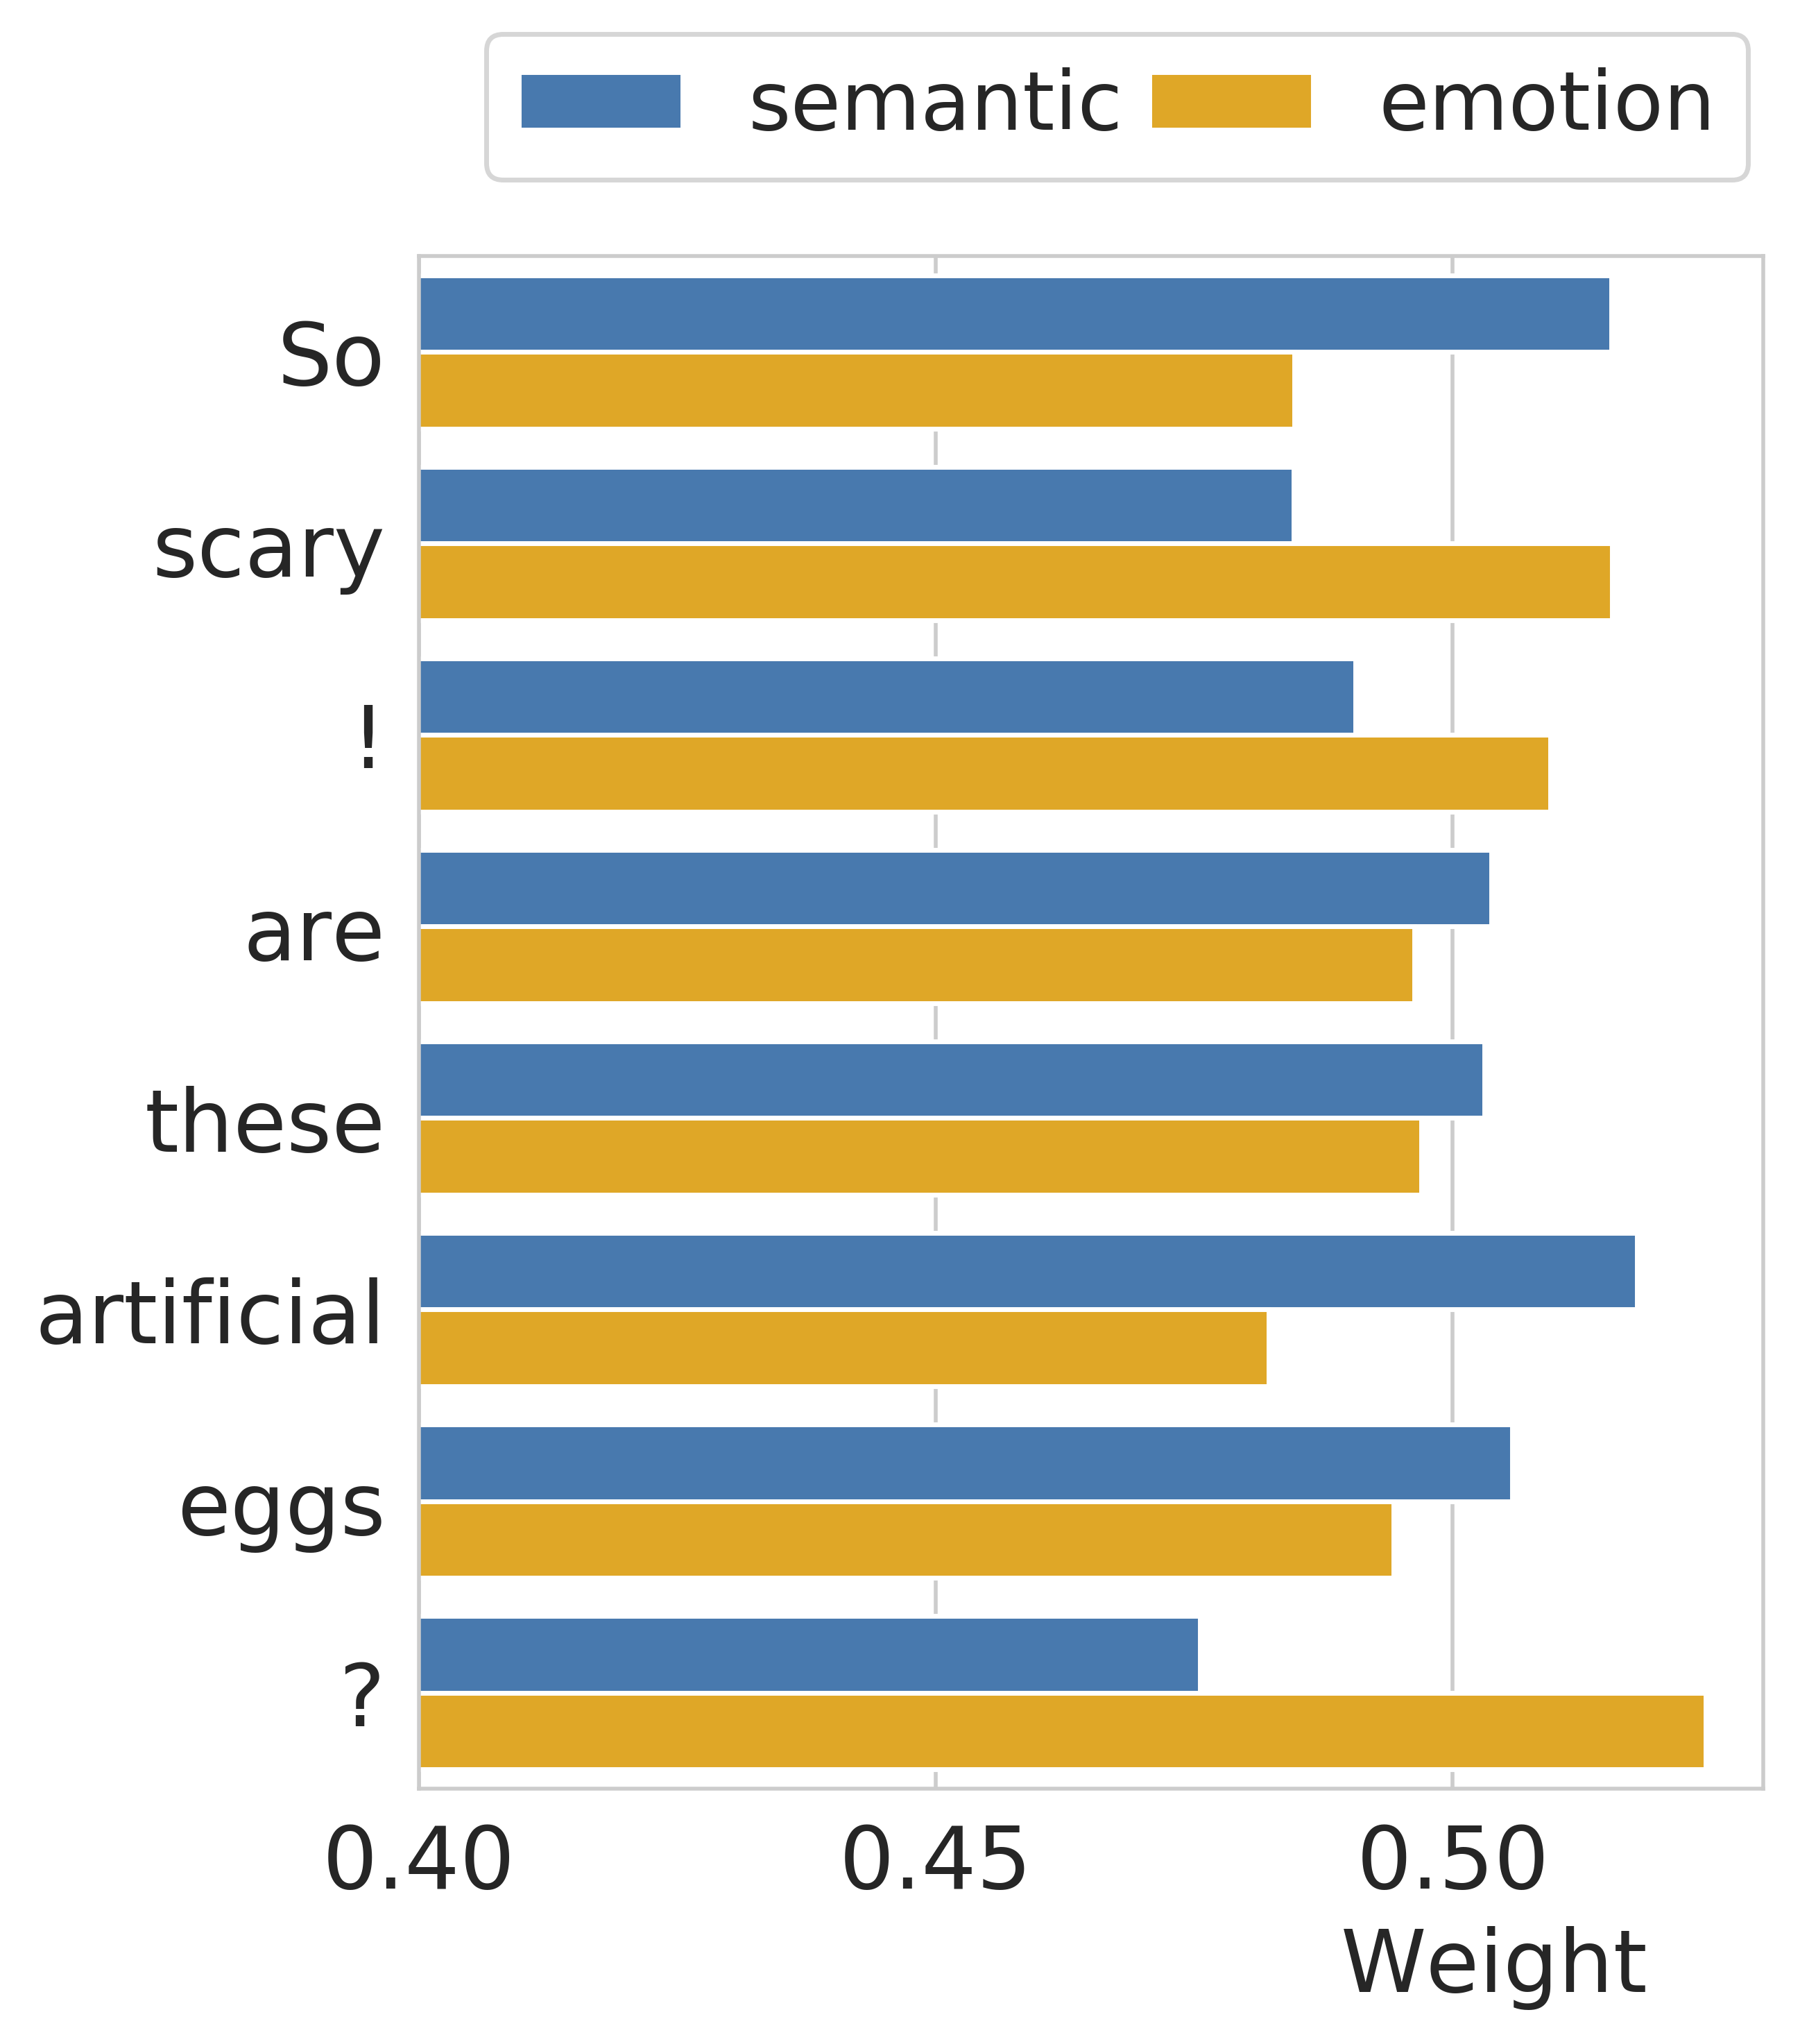
\includegraphics[width=0.45\textwidth]{./Figure/case1.png}
		\begin{minipage}[t]{0.45\textwidth}
			\subfloat[]{\label{Fig:case1_1}%%
				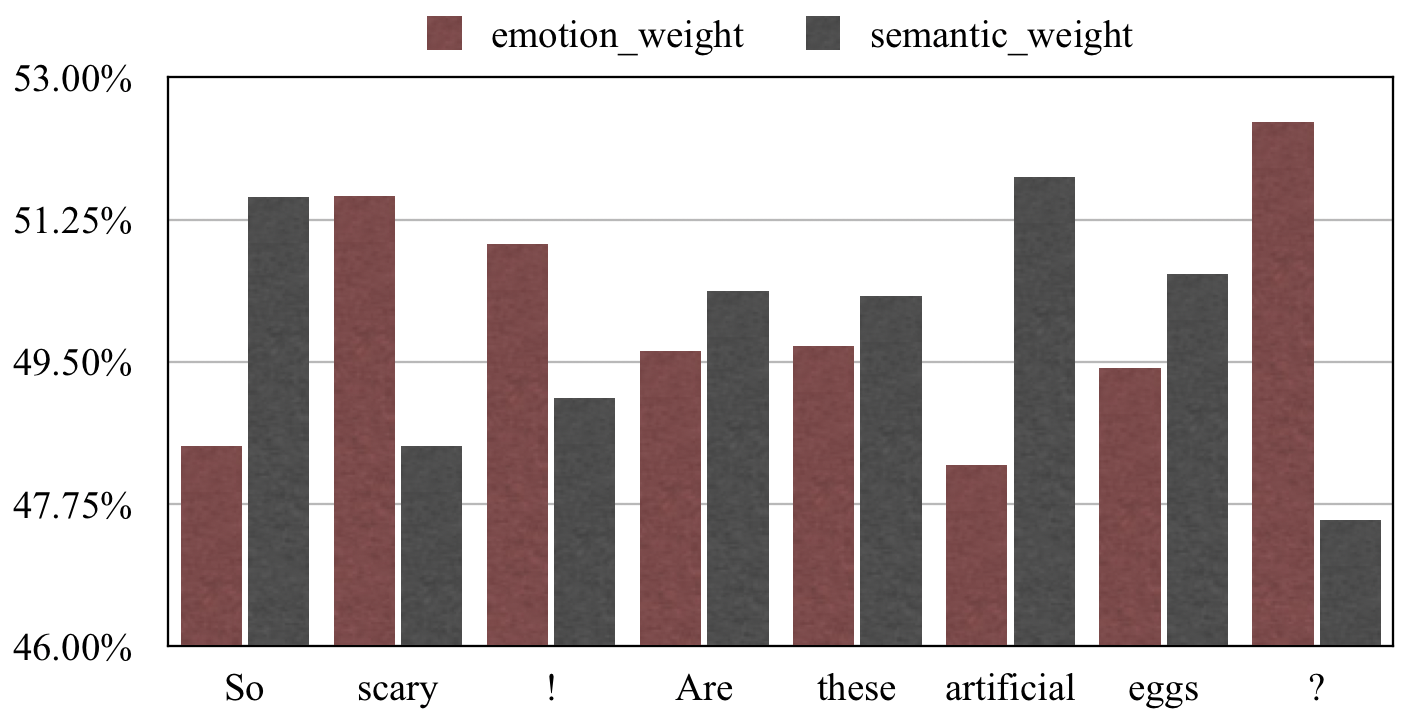
\includegraphics[width=3.2in]{./Figure/case1_1}}
		\end{minipage}
		\begin{minipage}[t]{0.45\textwidth}
			\subfloat[]{\label{Fig:case1_2}%%
				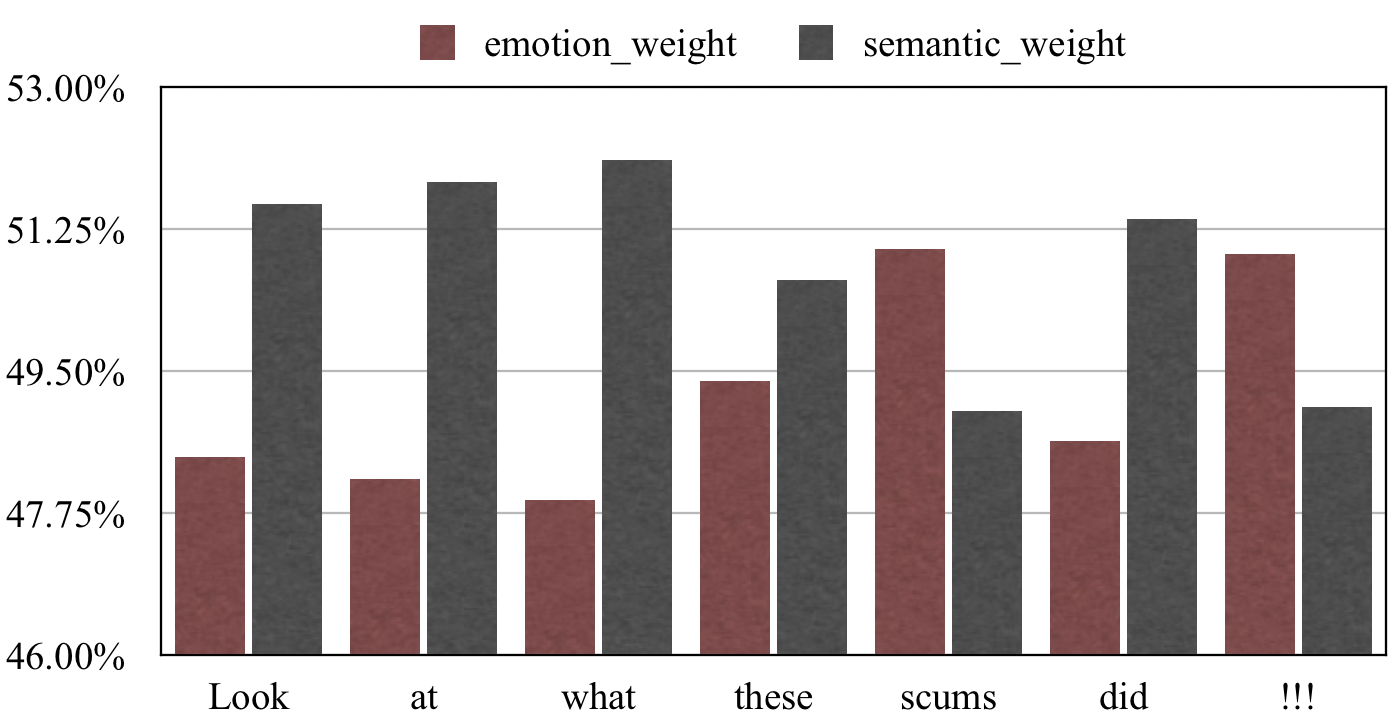
\includegraphics[width=3.2in]{./Figure/case1_2}}
		\end{minipage}
		\caption{The distribution of weights calculated by Gate\_C between semantic and emotion of each word in two sentences.}
		\label{Fig:case1}
	\end{figure}
	
	\subsection{Case Study}
	To further investigate what is actually learned behind gate units, we extract the vector $u_t$ in Gate\_C which is a weight vector between semantic vector $h_t^w$ and emotion vector $c_t^e$ for each word. We compute the average of the vector as an approximation of the weight between two modalities. Figure \ref{Fig:case1} shows two examples in fake news. We could observe that: 1) emotion part in sentiment words such as {\em "scary", "!" , "?"} and {\em "scums"} gains higher weight than semantic part. Many of these words even don't appear in sentiment dictionaries; and 2) sentiment words' emotion modalities obtain more attention than unemotional words.
	
	\begin{figure}[h]
		\centering
		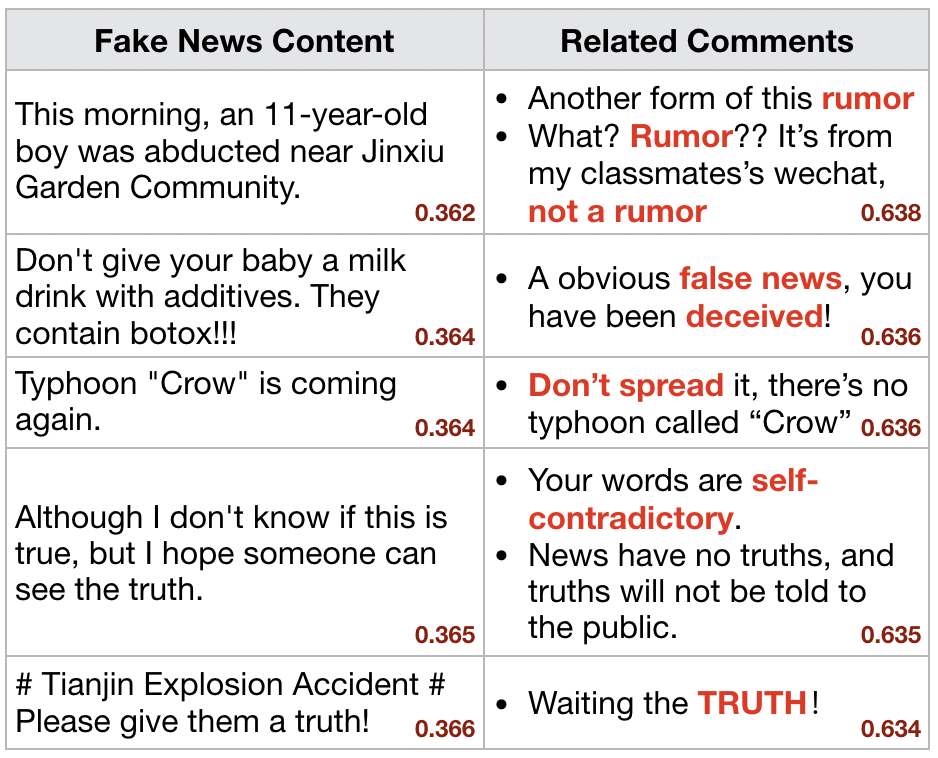
\includegraphics[width=0.45\textwidth]{./Figure/case2.png}
		\caption{Fake news whose comment modules are top weighed by Gate\_M.}
		\label{Fig:case2}
	\end{figure}
	
	Similarly, we also compute the average of vector $r$ as an approximation of weights between content module and comment module in Gate\_M. Figure \ref{Fig:case2} show 5 fake news pieces whose comment modules are top-weighted. Interestingly,  most of these news pieces' comments contains cues for verifying the truth of news content(e.g.,"deceived", "rumor"). This validates the capability of Gate\_M on capture important knowledge while fusing different modalities.
	
	\section{Conclusion}
	In this paper, we propose an end-to-end emotion-based fake news detection framework, {\m}, which incorporates publisher emotion and social emotion in fake news detection simultaneously. We apply content module and comment module to exploit semantic and emotion information from the publisher and users, respectively. Technically, we adopt embedding to capture emotion information for each word. To fully explore emotion in news event, three types of gates are proposed for fusion at different levels in {\m}. Extensive experiments on Weibo and Twitter datasets demonstrate that the proposed {\m} model is effective for detecting fake news and outperforms several state-of-art  fake news detection methods.
	
	
	\bibliographystyle{IEEEtran}
	\bibliography{IEEEexample}
	
	%\begin{thebibliography}{00}
	%\bibitem{b1} G. Eason, B. Noble, and I. N. Sneddon, ``On certain integrals of Lipschitz-Hankel type involving products of Bessel functions,'' Phil. Trans. Roy. Soc. London, vol. A247, pp. 529--551, April 1955.
	%\bibitem{b2} J. Clerk Maxwell, A Treatise on Electricity and Magnetism, 3rd ed., vol. 2. Oxford: Clarendon, 1892, pp.68--73.
	%\bibitem{b3} I. S. Jacobs and C. P. Bean, ``Fine particles, thin films and exchange anisotropy,'' in Magnetism, vol. III, G. T. Rado and H. Suhl, Eds. New York: Academic, 1963, pp. 271--350.
	%\bibitem{b4} K. Elissa, ``Title of paper if known,'' unpublished.
	%\bibitem{b5} R. Nicole, ``Title of paper with only first word capitalized,'' J. Name Stand. Abbrev., in press.
	%\bibitem{b6} Y. Yorozu, M. Hirano, K. Oka, and Y. Tagawa, ``Electron spectroscopy studies on magneto-optical media and plastic substrate interface,'' IEEE Transl. J. Magn. Japan, vol. 2, pp. 740--741, August 1987 [Digests 9th Annual Conf. Magnetics Japan, p. 301, 1982].
	%\bibitem{b7} M. Young, The Technical Writer's Handbook. Mill Valley, CA: University Science, 1989.
	%\end{thebibliography}
	
\end{document}
